\documentclass[11pt,a4paper,twocolumn,twoside]{article}
\usepackage[utf8]{inputenc}
\usepackage{multicol}
\usepackage{graphicx}
\usepackage{fancyhdr}
\usepackage{times}
\usepackage{titlesec}
\usepackage{multirow}
\usepackage{lettrine}
\usepackage{enumitem}
\usepackage{tabulary}
\usepackage{tabularx}
\usepackage{listings}
\usepackage{indentfirst}
\usepackage{url}
\usepackage{eurosym}
\usepackage{rotating}
\usepackage{longtable}
\usepackage{dblfloatfix}
\usepackage{booktabs}
\usepackage[sorting=none]{biblatex}
\usepackage[top=2.2cm, bottom=2.2cm, left=2cm, right=2cm]{geometry}
\usepackage[figurename=Fig.,tablename=TABLE]{caption}
\setlength{\parskip}{0.3em}
\addbibresource{Resources/refs.bib}

\newcommand\blfootnote[1]{%
  \begingroup
  \renewcommand\thefootnote{}\footnote{#1}%
  \addtocounter{footnote}{-1}%
  \endgroup
}

\fancyhead[RE]{\scriptsize Master in Computer Vision, CVC. Module 5: Visual Recognition}
\fancyhead[LO]{\scriptsize Master in Computer Vision, CVC. Module 5: Visual Recognition}
\fancyhead[RO]{\thepage}
\fancyhead[LE]{\thepage}
\fancyfoot[CO,CE]{}

\title{\Huge\sffamily Visual Recognition}
\author{Stanley Albayeros \texttt{stanley.albayeros@gmail.com}\and Alejandro Zarate \texttt{alejandro.zarate@e-campus.uab.cat}\and Oriol Catalan \texttt{oriol.catalan@e-campus.uab.cat} \and Victor Casales \texttt{victor.casales@e-campus.uab.cat}}

\date{Master in Computer Vision, CVC. Module 5: Visual Recognition March 2021}

\begin{document}
    
\fancypagestyle{primerapagina}
{
   \fancyhf{}
   \fancyhead[L]{\scriptsize Master in Computer Vision, CVC. Module 5: Visual Recognition}
   \fancyfoot[C]{\scriptsize March 2021, Centre de Visió per Computador (UAB) }
}
\pagestyle{fancy}

\twocolumn[\begin{@twocolumnfalse}
\begin{center}
    \maketitle
\parbox{0.8\textwidth}
{\sffamily
\textbf{Abstract --}In this final delivery of our laboratory results, we use Facebook's Detectron2 framework to analyze how modifying images can affect the performance of a model's capacity to properly detect objects in an image. We "attack" the model by transplanting objects from other images in a dataset, scaling and moving correctly detected objects within the same image and modifying the surroundings of a detected object to see how the model performs in these new situations.

\bigskip
\textbf{Keywords -- Detectron2, COCO Dataset, COCO, detection, machine learning, deep learning, cnn, mask r-cnn.}
}

\bigskip

{\vrule depth 0pt height 0.5pt width 4cm\hspace{7.5pt}%
\raisebox{-3.5pt}{\fontfamily{pzd}\fontencoding{U}\fontseries{m}\fontshape{n}\fontsize{11}{12}\selectfont\char70}%
\hspace{7.5pt}\vrule depth 0pt height 0.5pt width 4cm\relax}

\end{center}

\bigskip

\end{@twocolumnfalse}]


% \blfootnote{Stanley Albayeros: stanley.albayeros@gmail.com}
% \blfootnote{Alejandro Zarate: alejandro.zarate@e-campus.uab.cat}
% \blfootnote{Oriol Catalán: oriol.catalan@e-campus.uab.cat}
% \blfootnote{Víctor Casales: victor.casales@e-campus.uab.cat}


\section{Introduction}
\lettrine[lines=2]{D}etectron2, built by the Facebook AI Research team (FAIR)\cite{wu2019detectron2}, is a framework of libraries designed to support rapid implementation and evaluation of computer vision research. It includes implementations of popular object detection models such as Mask R-CNN and Faster R-CNN, already pre-trained and ready to use.

Object detection refers to the ability to identify some or all of the objects represented in an image by rough location and/or class. Object detection is usually signaled by bounding boxes (Fig.\ref{fig:Object_detection}).

\renewcommand{\headrulewidth}{1pt}

\begin{figure}[ht]
\centering
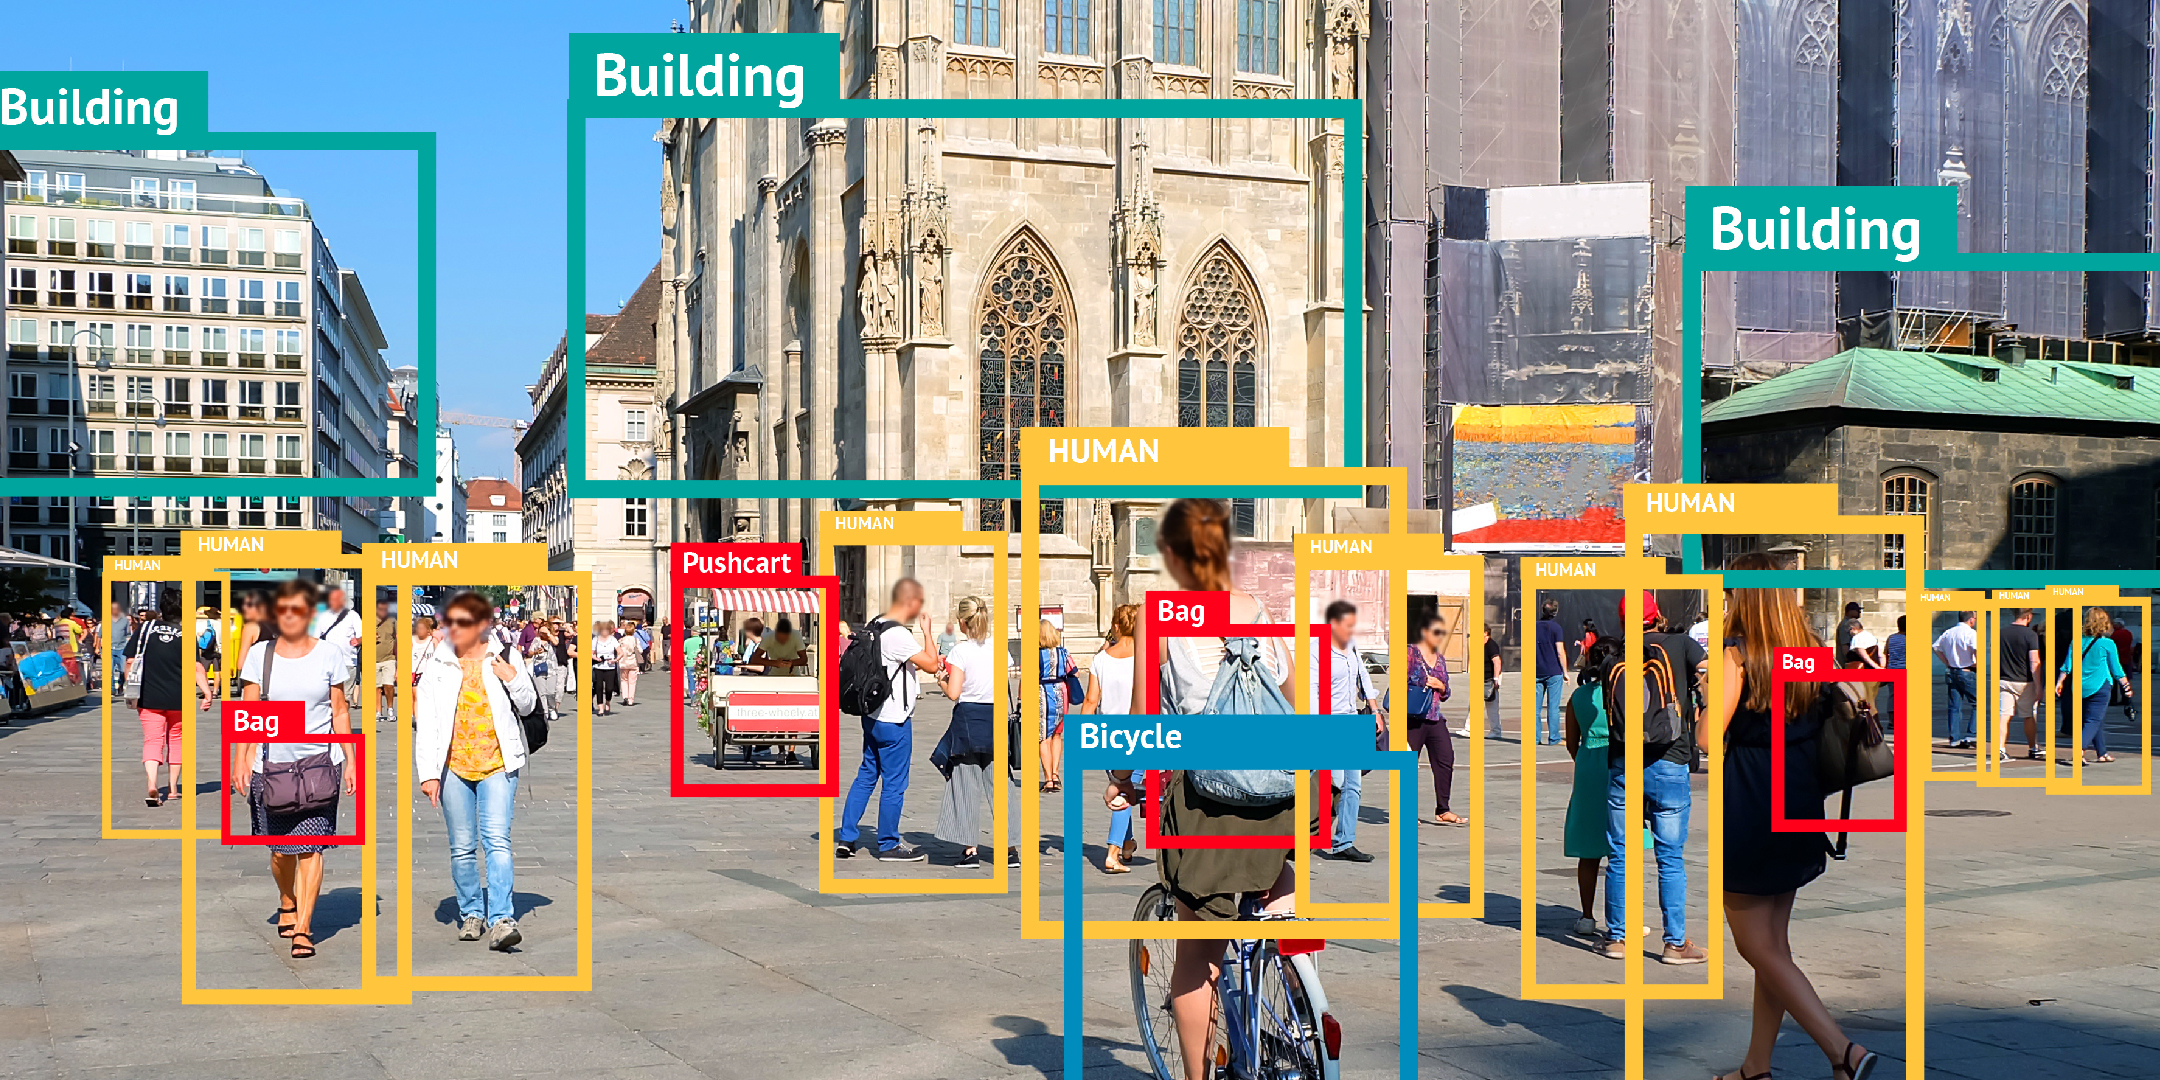
\includegraphics[width=0.9\linewidth]{Resources/Images/object_detection.jpg}
\caption{Object detection}
\label{fig:Object_detection}
\end{figure}

Object segmentation, also called semantic segmentation, seeks to create a per-pixel representation of the image in terms of the different objects or regions contained within(Fig. \ref{fig:Object_segmentation}). 

\begin{figure}[ht]
    \centering
    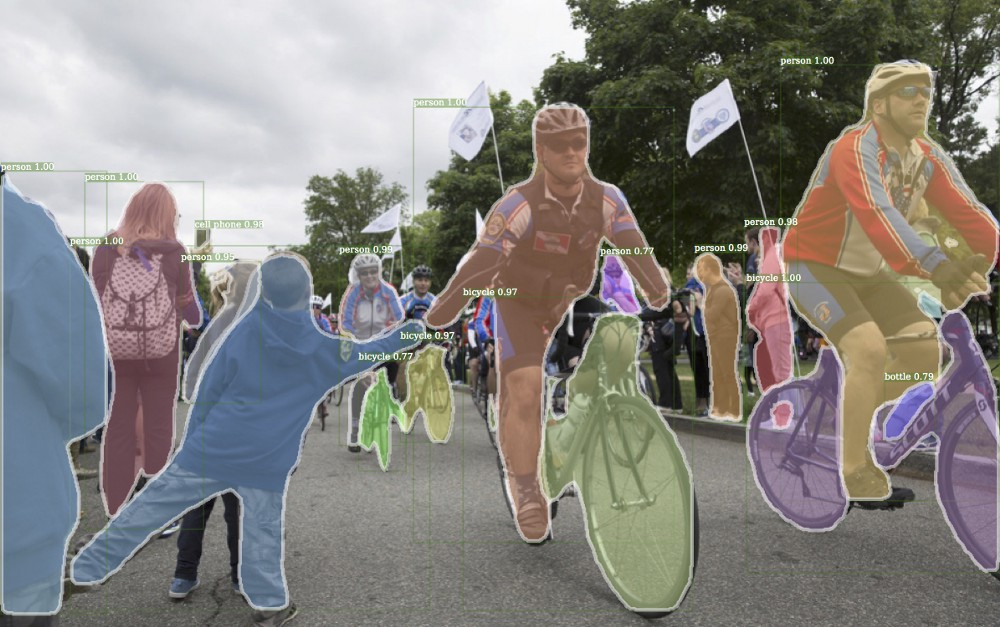
\includegraphics[width=0.8\linewidth]{Resources/Images/object_segmentation.jpg}
    \caption{Object segmentation}
    \label{fig:Object_segmentation}
    \end{figure}


\section{Fast history of Object detection}
\subsection{Region based CNN: R-CNNs}
Fast-forwarding to 2013, passing several improvements to compute power and the concepts used in CNNs. Uijlings et al.\cite{uijlings_van} proposed a method of generating possible object locations for use in object recognition. This allowed the creation of Region-based CNNs (R-CNNs).

R-CNNs have the downside of being slower than previous models, even though they require the use of pre-trained CNNs. This stems from the forward computations required from the CNN to perform object detection on our proposed regions. 

\subsection{Fast R-CNNs}

The R-CNN's needs to extract features for each proposed region indepently. This feature extraction process results in a high amount of repetitive and unneeded computations. To solve this, in 2015  Girshick\cite{girshick_2015} proposes the Fast R-CNN architecture. 

Compared to previous architectures, Girshick introduces Region of Interest (RoI) pooling, using the entire image as the original CNN input for feature extraction bypassing the region proposal method.

\subsection{Faster R-CNN}
The main issue with Fast R-CNNs is that they require a high amount of region proposals generated in the initial selective search. This is computationally expensive and, as with the original R-CNN, results in unnecessary computations.

The Faster R-CNN architecture, proposed by Shaoqin Ren, Kaiming He, Ross Girshick and Jian Sun\cite{ren_he_girshick_sun_2015} fixes this by replacing the selective search with a completely new neural network devoted solely to region proposal: a Region Proposal Network (RPN). With the RPN we predict a bounding boxes that are used as input regions. The RPN is trained along the re rest of the model and can lear to generate high quality proposed regions.

\subsection{Mask R-CNN}
On March 2017, Kaiming He et al.\cite{he_gkioxari_dollár_girshick_2017} published a second paper improving their architecture even further. Kaiming et al. extended the Faster R-CNN architecture following a similiar line of thought as they did with the RPN proposal: adding a convolutional network after the RoI aligned to locate objects at a pixel level within the image. This aditional CNN runs parallel with the bounding box detection and class prediction branches.

\subsection{Mesh R-CNN}
After mask R-CNNs, in 2019 Georgia Gkioxari, Jitendra Malik and Justin Johnson\cite{gkioxari_malik_johnson_2019} published a paper improving the pipeline to predict 3D shapes out of 2D images. They modify mask R-CNN in the same way the past two sections have done so: by introducing a new network to the pipeline. 

\section{Week 3: Using pre-trained models on new datasets}

This week we were tasked to perform several experiments using Faster R-CNN and RetinaNet pre-trained models on the KITTI-MOTS and MOTSChallenge datasets.

\subsection{The new datasets}

We are introduced to two new datasets to work on: MOTSChallenge and KITTI-MOTTS. MOTSChallenge is a dataset aimed at improving the performance of models when detecting pedestrians, it contains several sequences of sequential photographs. It is also used to train Multi-Object Tracking and Segmentation (MOTS). KITTI-MOTTS on the other hand, is a dataset aimed at improving both, pedestrian and vehicle detection.

The annotations of the datasets, although very complete, are not compatible with COCO's annotation format, so our first task was to write a script to translate the annotations to a COCO-compatible format.

\subsection{Qualitative and quantitative analysis}

For the qualitative tested several of the models contained in the COCO model library, and ended up favouring the $"101\_32x8d\_FPN\_3x"$ model for RCNN (Fig. \ref{fig:r50r101}) and the $"R\_50\_FPN\_1x"$ model for RetinaNet (Fig. \ref{fig:r50retina}).

\begin{figure}[ht]
    \centering
    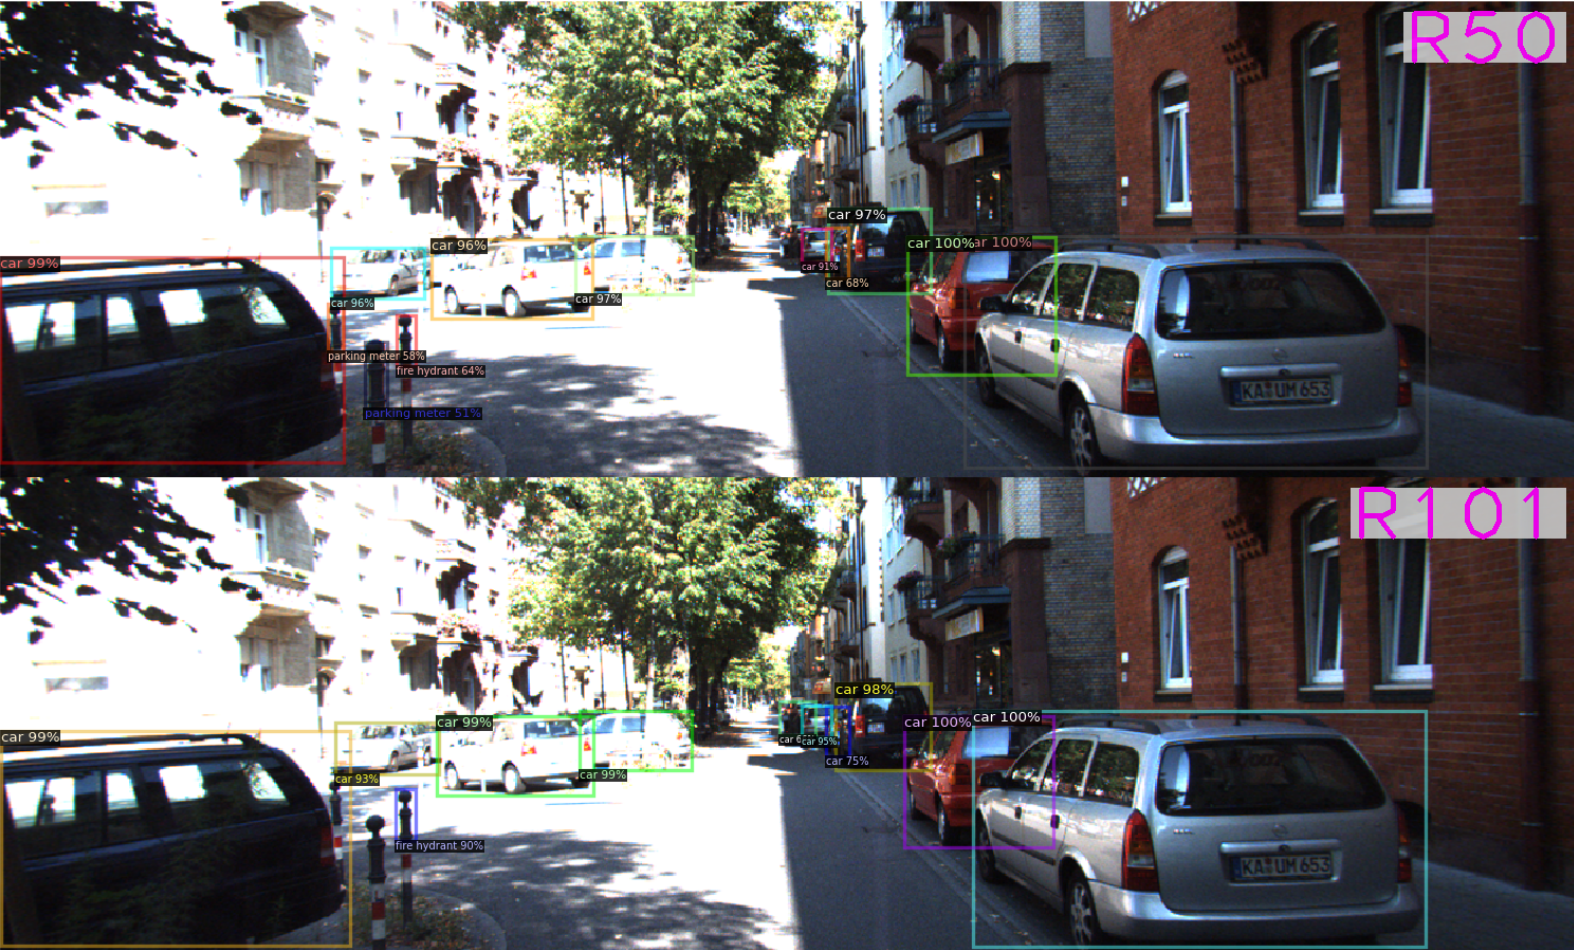
\includegraphics[width=0.8\linewidth]{Resources/Images/r50r101.png}
    \caption{RCNN samples.}
    \label{fig:r50r101}
    \end{figure}

\begin{figure}[ht]
    \centering
    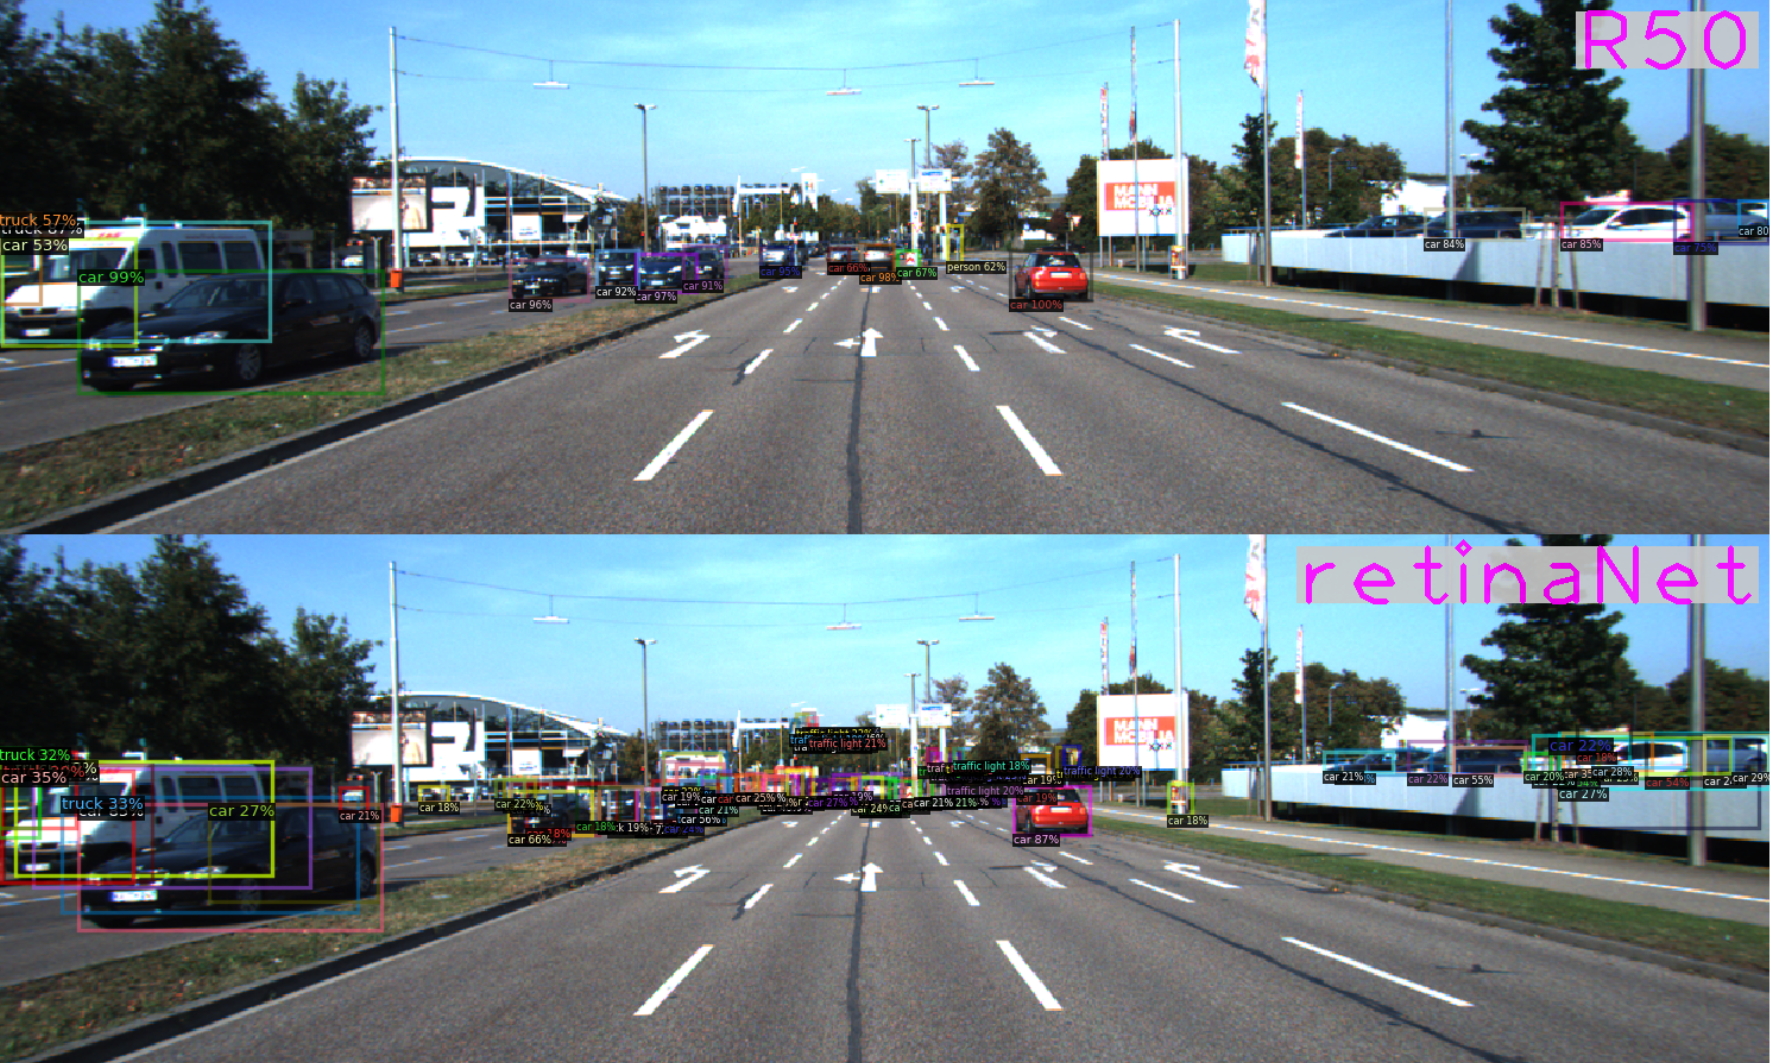
\includegraphics[width=0.8\linewidth]{Resources/Images/r50retina.png}
    \caption{RetinaNet samples.}
    \label{fig:r50retina}
    \end{figure}

Afterwards, we proceed to quantitatively analyse how these models perform on the validation of the KITTI-MOTS dataset. We used $AP_{(50)}$ metrics to compare the performance of the models, for both overall model performance and per-class performance (Table \ref{table:KITTI_Table1}.). 

\begin{table}[ht]
    \centering
    \begin{tabular}{|c || c | c|} 
        \hline
          & \textbf{R-CNN} & \textbf{RetinaNet} \\ [0.8ex] 
          \hline
         $AP_{(50)}$ & 0.415 & 0.461  \\ 
         \hline
         $AP_{(50)}$ Car & 0.576 & 0.553 \\
         \hline
         $AP_{(50)}$ Pedestrian & 0.456 & 0.397 \\
         \hline
    \end{tabular}
    \caption{\label{table:KITTI_Table1}Pre-trained $AP_{(50)}$ on KITTI-MOTS validation.}
\end{table}

Both models preform adequately for Car objects, but the Pedestrian class has an impact on the performance obtained, especially on RetinaNet which takes a larger drop in performance than RCNN.

\subsection{Quantitative analysis after training on new datasets.}

For this experiment, we split each dataset into training ($60\%$), validation ($20\%$), and test ($20\%$). Our testing parameters were: learning rate = {0.0001, 0.001, 0.01}, ROI proposals = {32,64,128} at 1000 iterations.

The collected data for the RCNN model (Table \ref{table:RCNN_Table_training}) and revealed that, for all our experiments, RetinaNet provided much lower results compared to the pre-trained models used in mentioned before, which we infer we did not implement our test cycle properly for RetinaNet. The results were above 15\% performance drop and were not included in the table.

\begin{table}[ht]
    \centering
    \begin{tabular}{|c | c || c|} 
        \hline
        \textbf{LR} & \textbf{ROIs} & \textbf{$AP_{(50)}$} \\ [0.8ex] 
            \hline
            0.0001 & 32 & 0.236 \\ 
            \hline
            0.0001 & 64 & 0.371\\ 
            \hline
            0.0001 & 128 & 0.394 \\ 
            \hline
            0.001 & 32 & 0.410\\ 
            \hline
            0.001 & 64 & 0.467\\ 
            \hline
            \textbf{0.001} & \textbf{128} & \textbf{0.572}\\ 
            \hline
            0.01 & 32 & 0.365\\ 
            \hline
            0.01 & 64 & 0.379\\ 
            \hline
            0.01 & 128 & 0.426\\ 
         \hline
    \end{tabular}
    \caption{\label{table:RCNN_Table_training}RCNN Training.}
\end{table}

\subsection{Evaluating on KITTI-MOTS test set}

We took the best performing model after the last section and used it on the official KITTI-MOTS test set with the following parameters: LR = 0.001, ROI Batch=128 trained model was selected. 


\begin{table}[ht]
    \centering
    \begin{tabular}{|c || c |} 
        \hline
          & \textbf{R-CNN}\\ [0.8ex] 
          \hline
         $AP_{(50)}$ & 0.331\\ 
         \hline
         $AP_{(50)}$ Car & 0.421\\
         \hline
         $AP_{(50)}$ Pedestrian & 0.367\\
         \hline
    \end{tabular}
    \caption{\label{table:KITTI-MOTS-FINAL}Final model $AP_{(50)}$ on KITTI-MOTS validation.}
\end{table}

As seen in Table \ref{table:KITTI-MOTS-FINAL}, our results were noticeably worse than the obtained with pre-trained model's, even though our model outperformed them with our dataset split. This may be due to the images in the test set benefiting from the higher region count for this model.

\section{Week 4: Object Segmentation}

We were tasked with developing segmentation techniques with different networks and we decided to combine object detection and object segmentation techniques.
We also needed to provide in our ground truth dictionary the information of the segmented instances with the COCO notation.

\subsection{Inference on KITTI-MOTS with Mask-RCNN}

We analyzed the inference performance obtained with different number of layers of the pre-trained Mask-RCNN models with the KITTI-MOTS validation set and the performance obtained with two pre-trained models using different datasets (COCO dataset and 'COCO and Cityscapes'). The results obtained from the pre-trained models with both datasets are shown in Table \ref{table:week4_taskA_COCO} in the Annex. For C4 models we noticed almost no difference between them, they were also the slowest at inference. For DC5 we appreciated a slight drop in AP but had a faster inference time, as they improve their AP:Time ratio notably in exchange for a slight performance drop. Finally, FPN were the most efficient, displaying excellent AP:Time ratios.

AP:Time ratio will be used to choose the models to use on the next sections, as it allows us to find a faster-to-train model with no performance compromise.


\subsection{Training with different datasets}
For this experiment we trained different models using different datasets. For the sake of consistency, they were all evaluated with KITTI-MOTS validation set. The results can be seen on the tables listed below, we only segmentation results were as bbox detection was not this week's focus.

\begin{itemize}
    \item COCO + KITTI-MOTS (Table \ref{table:task_b_COCO_kittimots})
    \item COCO + KITTI-MOTS + MOTSChallenge (Table \ref{table:task_b_COCO_motschallenge})
    \item COCO + Cityscapes + KITTI-MOTS (Table \ref{table:task_b_coco_cityscapes_kittimots_motschallenge})
    \item COCO + Cityscapes + KITTI-MOTS + MOTSChallenge (Table \ref{table:task_b_coco_cityscapes_kittimots_motschallenge})
\end{itemize}

From the results, we can see that KITTI-MOTTS favors the model's AP when detecting cars, while MOTSChallenge favors pedestrian detection. Cityscapes provides a boost to both classes' AP values. 
\subsection{Optimizing Hyperparameters}
Our hyperparameter selection was tested on the R50-FPN-x3 model, since it had the best performing AP to time ratio and would let us run tests faster while providing good results.
\begin{itemize}
    \item IOU THRESHOLDS([0.4, 0.6]- [0.4, 0.6] - [0.4, 0.8]))
    \item ANCHOR-GENERATOR.SIZES ([64, 128, 256, 512,1024]] - [[32, 64, 128, 256, 512])
    \item ANCHOR-GENERATOR.ASPECT-RATIOS ([[0.5, 1.0, 2.0]] - [[0.25, 0.5, 1.0]])
\end{itemize}
A 10 pt increase to AP at the cost of half a minute of training more than the results before was satisfactory. The model trains fast and performs noticeably better than the pre-trained one in Model Zoo. Even though an untrained X101-FPN-x3 performs similarly and is faster, the R50 model took up to ~6GB of VRAM on the longest testing run, using MOTSChallenge+KITTI-Mots, while the X101 model couldn't fit a 10GB GPU.  \newpage
  
  
\section{Week 5: Breaking models}

\subsection{Lab Introduction}

On this final week, we are tasked with trying to break pre-trained models. The main objective is to test out how these models perform against intentionally manipulated images, following the footsteps of Amir Rosenfeld's paper "The Elephant in the Room"\cite{elephantroom}.


\subsection{New dataset: Out-Of-Context}
We are introduced to a new dataset: Out-Of-Context. These are images of seemingly mundane situations where objects are not being used or exist on their normally occurring places. We use Faster R-CNN (R50-FPN-3x) for bounding boxes and Mask R-CNN (R50-FPN-3x) for segmentation. The model was chosen for it's speed and reliability, as we discussed in the previous week.

\subsection{Using pre-trained models on the new dataset}
For this task, we start by taking the model and running predictions on the whole dataset. As we don't have annotations for this dataset, we take these predictions, and build a co-occurrence matrix of the classes to have some sort of baseline performance of the model (Fig.\ref{fig:task_a_cooc} found in Annex).

Many of these objects have different textures, or relative sizes that are not "normal" on photographs, so the model misses objects in the dataset that it wouldn't otherwise miss if they were more "normal". Fig. \ref{fig:theater}, for example, shows that the model detected only one person on a theater packed with people. 


\begin{figure}[htb]
    \centering
    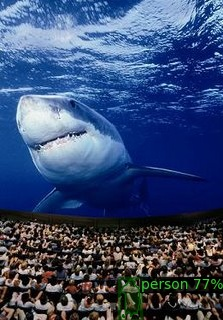
\includegraphics[height=0.8\linewidth]{Resources/Images/im029.jpg}
    \caption{Covid-compliant theater.}
    \label{fig:theater}
    \end{figure}


\subsection{Analyzing performance of the models on modified images}
On the following three tasks, we perform a series of modifications to images of the COCO dataset to see how the model performs. We use the 2017 training dataset. As the modifications are done mostly manually, we take random samples of images from this dataset.

\subsubsection{Transplanting new objects}
For this task, we have selected properly identified objects from the “coco 2017 train” dataset and placed them randomly on other images from the same dataset. We selected a small randomly sampled subset of 25 images from the "coco 2017 train" dataset to make qualitative analysis simpler, as the transplanting of objects was not automated. On this task, we take objects detected from images in the COCO dataset and transplant them into other images. These objects are "out-of-context" in relation to the images we are transplanting them to. 

To help in the quantitative analysis, we generated the co-ocurrence matrix that you can find in the annex (Fig. \ref{fig:task_b_cooc}

As an interesting note, it is fun to see how related items have high co-occurrences amongst them (Fig. \ref{fig:task_b_interesting}. There is a high co-occurrence amongst the classes: person, bottle, wine glass, cup, bowl, sandwich and dining table. These come from photographs of parties, diners, kitchens and social gatherings.


For our quantitative analysis, we consider the model’s inference on an unmodified image as 1, and value the decrease (or increase) in performance of the model’s inference on the modified images in a range of 0-1. We notice a decline in overall performance of the model, the trade-offs in images where new objects are detected are not enough to offset objects lost when transplanted objects occlude existing ones (See Fig. \ref{fig:task_b_deltas} in the Annex). 

\subsubsection{Qualitatively Transplant Existing Objects}
For this task, we transplanted objects within the same photo to see the effects on detection. We made a co-occurrence matrix for before(Fig. \ref{}) and after(Fig. \ref{fig:task_c_mod}) the transplant. Unlike task B, we did not get “new” classes on the modified sample of the dataset.

The worst effect of these transplants was that the transplanted object stopped being classified. Normally “big” objects like horse and people did not have this issue, but normally “small” objects like a bird stopped getting caught by the detector.

\begin{figure}[htb]
    \centering
    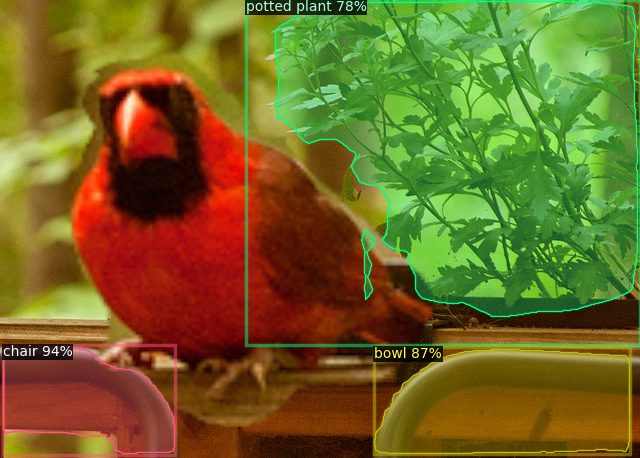
\includegraphics[height=0.8\linewidth]{Resources/Images/not_bird.png}
    \caption{Not a bird anymore}
    \label{fig:bird}
    \end{figure}
    
We also performed the same analysis as on task B for this task. Accuracy has taken a greater hit after transplanting and transforming objects within the photo. Even though some classes showed robustness, the dependance on relative size of the object in relation to the complete image seems to have affected a lot of the results, like the bird class. (Refer to Fig. \ref{fig:task_c_deltas}.)


\subsubsection{Feature interference according to Co-occurrence of
objects}

For the last task, we are to try to interfere with the model’s detection capabilities by taking features it correctly detected previously, and creating situations where it might not detect them anymore, or the confidence in the classes is lower

We randomly selected three new photos from the coco 2017 train dataset for this task, and applied 4 feature interferences to each one of them with masks, and one additional translation interference per each one of them. The modifications applied were: (2) random color noise, (3,4) 2 black/white gradients, (5) Gaussian blur + color difference outside the object’s mask and (6) translating the object using the random color noise as background (Refer to Figs.\ref{fig:task_d_bird}, \ref{fig:task_d_bear}, \ref{fig:task__cat} in the Annex).

From what we can tell, the model's bird detection is very strong (Fig.\ref{fig:task_d_bird}). We assume that if we were to “blow up” the size of the bird, the model would fail like one of the previous tasks, but we wanted to apply the same modifications to all images. Translation + noise lowered the bird’s confidence rating.

We did not manage to “break” the model’s ability to detect bears (Fig.\ref{fig:task_d_bear}). The segmentation mask does suffer on all of the modifications we made, as the bear in the middle’s segmentation mask encroaches on the top bear’s position on every modification.


A gradient makes our model detect the cat’s whiskers as airplanes (Fig.\ref{fig:task__cat}). The model reported a higher confidence score on all of our modifications than on the unmodified image. 




%   \newpage
\printbibliography








\newpage
\onecolumn
\section{Annex}


\begin{table}[hbt]
\centering
\resizebox{\columnwidth}{!}{\begin{tabular}{@{}llrr@{}}
\toprule
                                   &                                   & \multicolumn{1}{l}{R50-FPN\_x3} & \multicolumn{1}{l}{R50-DC5\_x3} \\ \midrule
\multicolumn{1}{|l|}{AP}           & \multicolumn{1}{l|}{bbox}         & \multicolumn{1}{r|}{59,30}      & \multicolumn{1}{r|}{55,41}      \\ \midrule
\multicolumn{1}{|l|}{AP}           & \multicolumn{1}{l|}{segmentation} & \multicolumn{1}{r|}{52,99}      & \multicolumn{1}{r|}{47,94}      \\ \midrule
\multicolumn{1}{|l|}{AP50}         & \multicolumn{1}{l|}{bbox}         & \multicolumn{1}{r|}{80,46}      & \multicolumn{1}{r|}{79,99}      \\ \midrule
\multicolumn{1}{|l|}{AP50}         & \multicolumn{1}{l|}{segmentation} & \multicolumn{1}{r|}{79,27}      & \multicolumn{1}{r|}{76,99}      \\ \midrule
\multicolumn{1}{|l|}{AP-Person}    & \multicolumn{1}{l|}{bbox}         & \multicolumn{1}{r|}{51,40}      & \multicolumn{1}{r|}{46,12}      \\ \midrule
\multicolumn{1}{|l|}{AP-Person}    & \multicolumn{1}{l|}{segmentation} & \multicolumn{1}{r|}{39,81}      & \multicolumn{1}{r|}{31,66}      \\ \midrule
\multicolumn{1}{|l|}{AP-Car}       & \multicolumn{1}{l|}{bbox}         & \multicolumn{1}{r|}{67,19}      & \multicolumn{1}{r|}{64,69}      \\ \midrule
\multicolumn{1}{|l|}{AP-Car}       & \multicolumn{1}{l|}{segmentation} & \multicolumn{1}{r|}{66,16}      & \multicolumn{1}{r|}{64,22}      \\ \midrule
\multicolumn{1}{|l|}{Elapsed Time} & \multicolumn{1}{l|}{}             & \multicolumn{1}{r|}{348,38}     & \multicolumn{1}{r|}{651,98}     \\ \midrule
ratio AP:Time                      &                                   & 5,88                            & 11,77                           \\ \bottomrule

\end{tabular}}

\caption{Trained on COCO + KITTI-MOTS datasets and validate on KITTI-MOTS}
\label{table:task_b_COCO_kittimots}
\end{table}

\begin{table*}[hbt]
    \centering
\begin{tabularx}{\textwidth}{|l|l|r|r|} \cline{1-4}
              &              & \multicolumn{1}{l|}{R50-FPN\_x3} & \multicolumn{1}{l|}{R50-DC5\_x3} \\ \cline{1-4}
AP            & bbox         & 58,63                            & 56,44                            \\ \cline{1-4}
AP            & segmentation & 53,53                            & 50,02                            \\ \cline{1-4}
AP50          & bbox         & 79,48                            & 80,06                            \\ \cline{1-4}
AP50          & segmentation & 77,37                            & 77,36                            \\ \cline{1-4}
AP-Person     & bbox         & 51,62                            & 49,69                            \\ \cline{1-4}
AP-Person     & segmentation & 41,60                            & 37,90                            \\ \cline{1-4}
AP-Car        & bbox         & 65,63                            & 63,19                            \\ \cline{1-4}
AP-Car        & segmentation & 65,45                            & 62,14                            \\ \cline{1-4}
Elapsed Time  &              & 407,87                           & 772,37                           \\ \cline{1-4}
ratio AP:Time &              & 6,96                             & 13,69                            \\ \cline{1-4} 
\end{tabularx}
\caption{\label{table:task_b_COCO_motschallenge}Trained on COCO + KITTI-MOTS + MOTSChallenge datasets and validate on KITTI-MOTS.}
\end{table*}

\begin{table*}[hbt]
\centering
\begin{tabularx}{\textwidth}{|l|l|r|r|} \cline{1-4}
              &               & \multicolumn{1}{l|}{C + K} & \multicolumn{1}{l|}{C + K + M} \\ \cline{1-4}
AP            & bbox          & 63,10                      & 61,13                          \\ \cline{1-4}
AP            & segmentation  & 56,70                      & 55,81                          \\ \cline{1-4}
AP50          & bbox          & 83,41                      & 82,27                          \\ \cline{1-4}
AP50          & segmentation  & 81,99                      & 79,72                          \\ \cline{1-4}
AP-Person     & bbox          & 55,64                      & 56,34                          \\ \cline{1-4}
AP-Person     & segmentation  & 41,64                      & 41,94                          \\ \cline{1-4}
AP-Car        & bbox          & 70,57                      & 65,91                          \\ \cline{1-4}
AP-Car        & segmentation  & 71,77                      & 69,68                          \\ \cline{1-4}
Elapsed Time  & Elapsed Time  & 711,94                     & 693,96                         \\ \cline{1-4}
ratio AP:Time & ratio AP:Time & 11,28                      & 11,35                          \\ \cline{1-4} 
\end{tabularx}
\caption{\label{table:task_b_coco_cityscapes_kittimots_motschallenge}Using Cityscapes data on coco + (K)ITTI or Coco + (K)ITTI + (M)OTSChallenge.}
\end{table*}

\begin{table*}[hbt]
\centering
\begin{tabularx}{\textwidth}{lcccccc}
\cline{1-7}
                                            & \multicolumn{1}{l}{\textbf{AP}} & \multicolumn{1}{l}{\textbf{AP50}} & \multicolumn{1}{l}{\textbf{AP-Person}} & \multicolumn{1}{l}{\textbf{AP-Car}} & \multicolumn{1}{l}{\textbf{Elapsed Time}} & \multicolumn{1}{l}{\textbf{ratio AP:Time}} \\ \cline{1-7}
\multicolumn{1}{|l|}{\textbf{R50-FPN\_x3}}  & \multicolumn{1}{c|}{53,02}      & \multicolumn{1}{c|}{80,72}        & \multicolumn{1}{c|}{38,44}             & 67,6                                & 195,42                                    & 4,68                                       \\ \cline{1-7}
\multicolumn{1}{|l|}{\textbf{R50-FPN\_x1}}  & \multicolumn{1}{c|}{50,98}      & \multicolumn{1}{c|}{79,93}        & \multicolumn{1}{c|}{36,22}             & 65,73                               & 215,17                                    & 10,51                                      \\ \cline{1-7}
\multicolumn{1}{|l|}{\textbf{R101-FPN\_x3}} & \multicolumn{1}{c|}{51,43}      & \multicolumn{1}{c|}{78,35}        & \multicolumn{1}{c|}{36,59}             & 66,27                               & 220,54                                    & 6,40                                       \\ \cline{1-7}
\multicolumn{1}{|l|}{\textbf{City-R50-FPN}} & \multicolumn{1}{c|}{50,05}      & \multicolumn{1}{c|}{77,21}        & \multicolumn{1}{c|}{36,85}             & 63,26                               & 259,8                                     & 3,85                                       \\ \cline{1-7}
\multicolumn{1}{|l|}{\textbf{X101-FPN\_x3}} & \multicolumn{1}{c|}{54,09}      & \multicolumn{1}{c|}{80,83}        & \multicolumn{1}{c|}{39,52}             & 68,66                               & 300,51                                    & 10,00                                      \\ \cline{1-7}
\multicolumn{1}{|l|}{\textbf{R50-DC5\_x3}}  & \multicolumn{1}{c|}{48,77}      & \multicolumn{1}{c|}{79,1}         & \multicolumn{1}{c|}{33,69}             & 63,84                               & 335,89                                    & 9,65                                       \\ \cline{1-7}
\multicolumn{1}{|l|}{\textbf{R101-DC5\_x3}} & \multicolumn{1}{c|}{49,28}      & \multicolumn{1}{c|}{78,6}         & \multicolumn{1}{c|}{33,88}             & 64,69                               & 360,62                                    & 6,41                                       \\ \cline{1-7}
\multicolumn{1}{|l|}{\textbf{R50-DC5\_x1}}  & \multicolumn{1}{c|}{45,88}      & \multicolumn{1}{c|}{76,98}        & \multicolumn{1}{c|}{29,97}             & 61,79                               & 344,06                                    & 6,00                                       \\ \cline{1-7}
\multicolumn{1}{|l|}{\textbf{R50-C4\_x3}}   & \multicolumn{1}{c|}{48,99}      & \multicolumn{1}{c|}{79,4}         & \multicolumn{1}{c|}{34,49}             & 63,49                               & 551,45                                    & 3,79                                       \\ \cline{1-7}
\multicolumn{1}{|l|}{\textbf{R50-C4\_x1}}   & \multicolumn{1}{c|}{47,59}      & \multicolumn{1}{c|}{79,28}        & \multicolumn{1}{c|}{32,97}             & 62,22                               & 568,38                                    & 3,32                                       \\\cline{1-7}
\end{tabularx}
\caption{Pre-trained $AP_{(50)}$ on KITTI-MOTS validation}
\label{table:week4_taskA_COCO}
\end{table*}


\begin{figure}[hbt]
    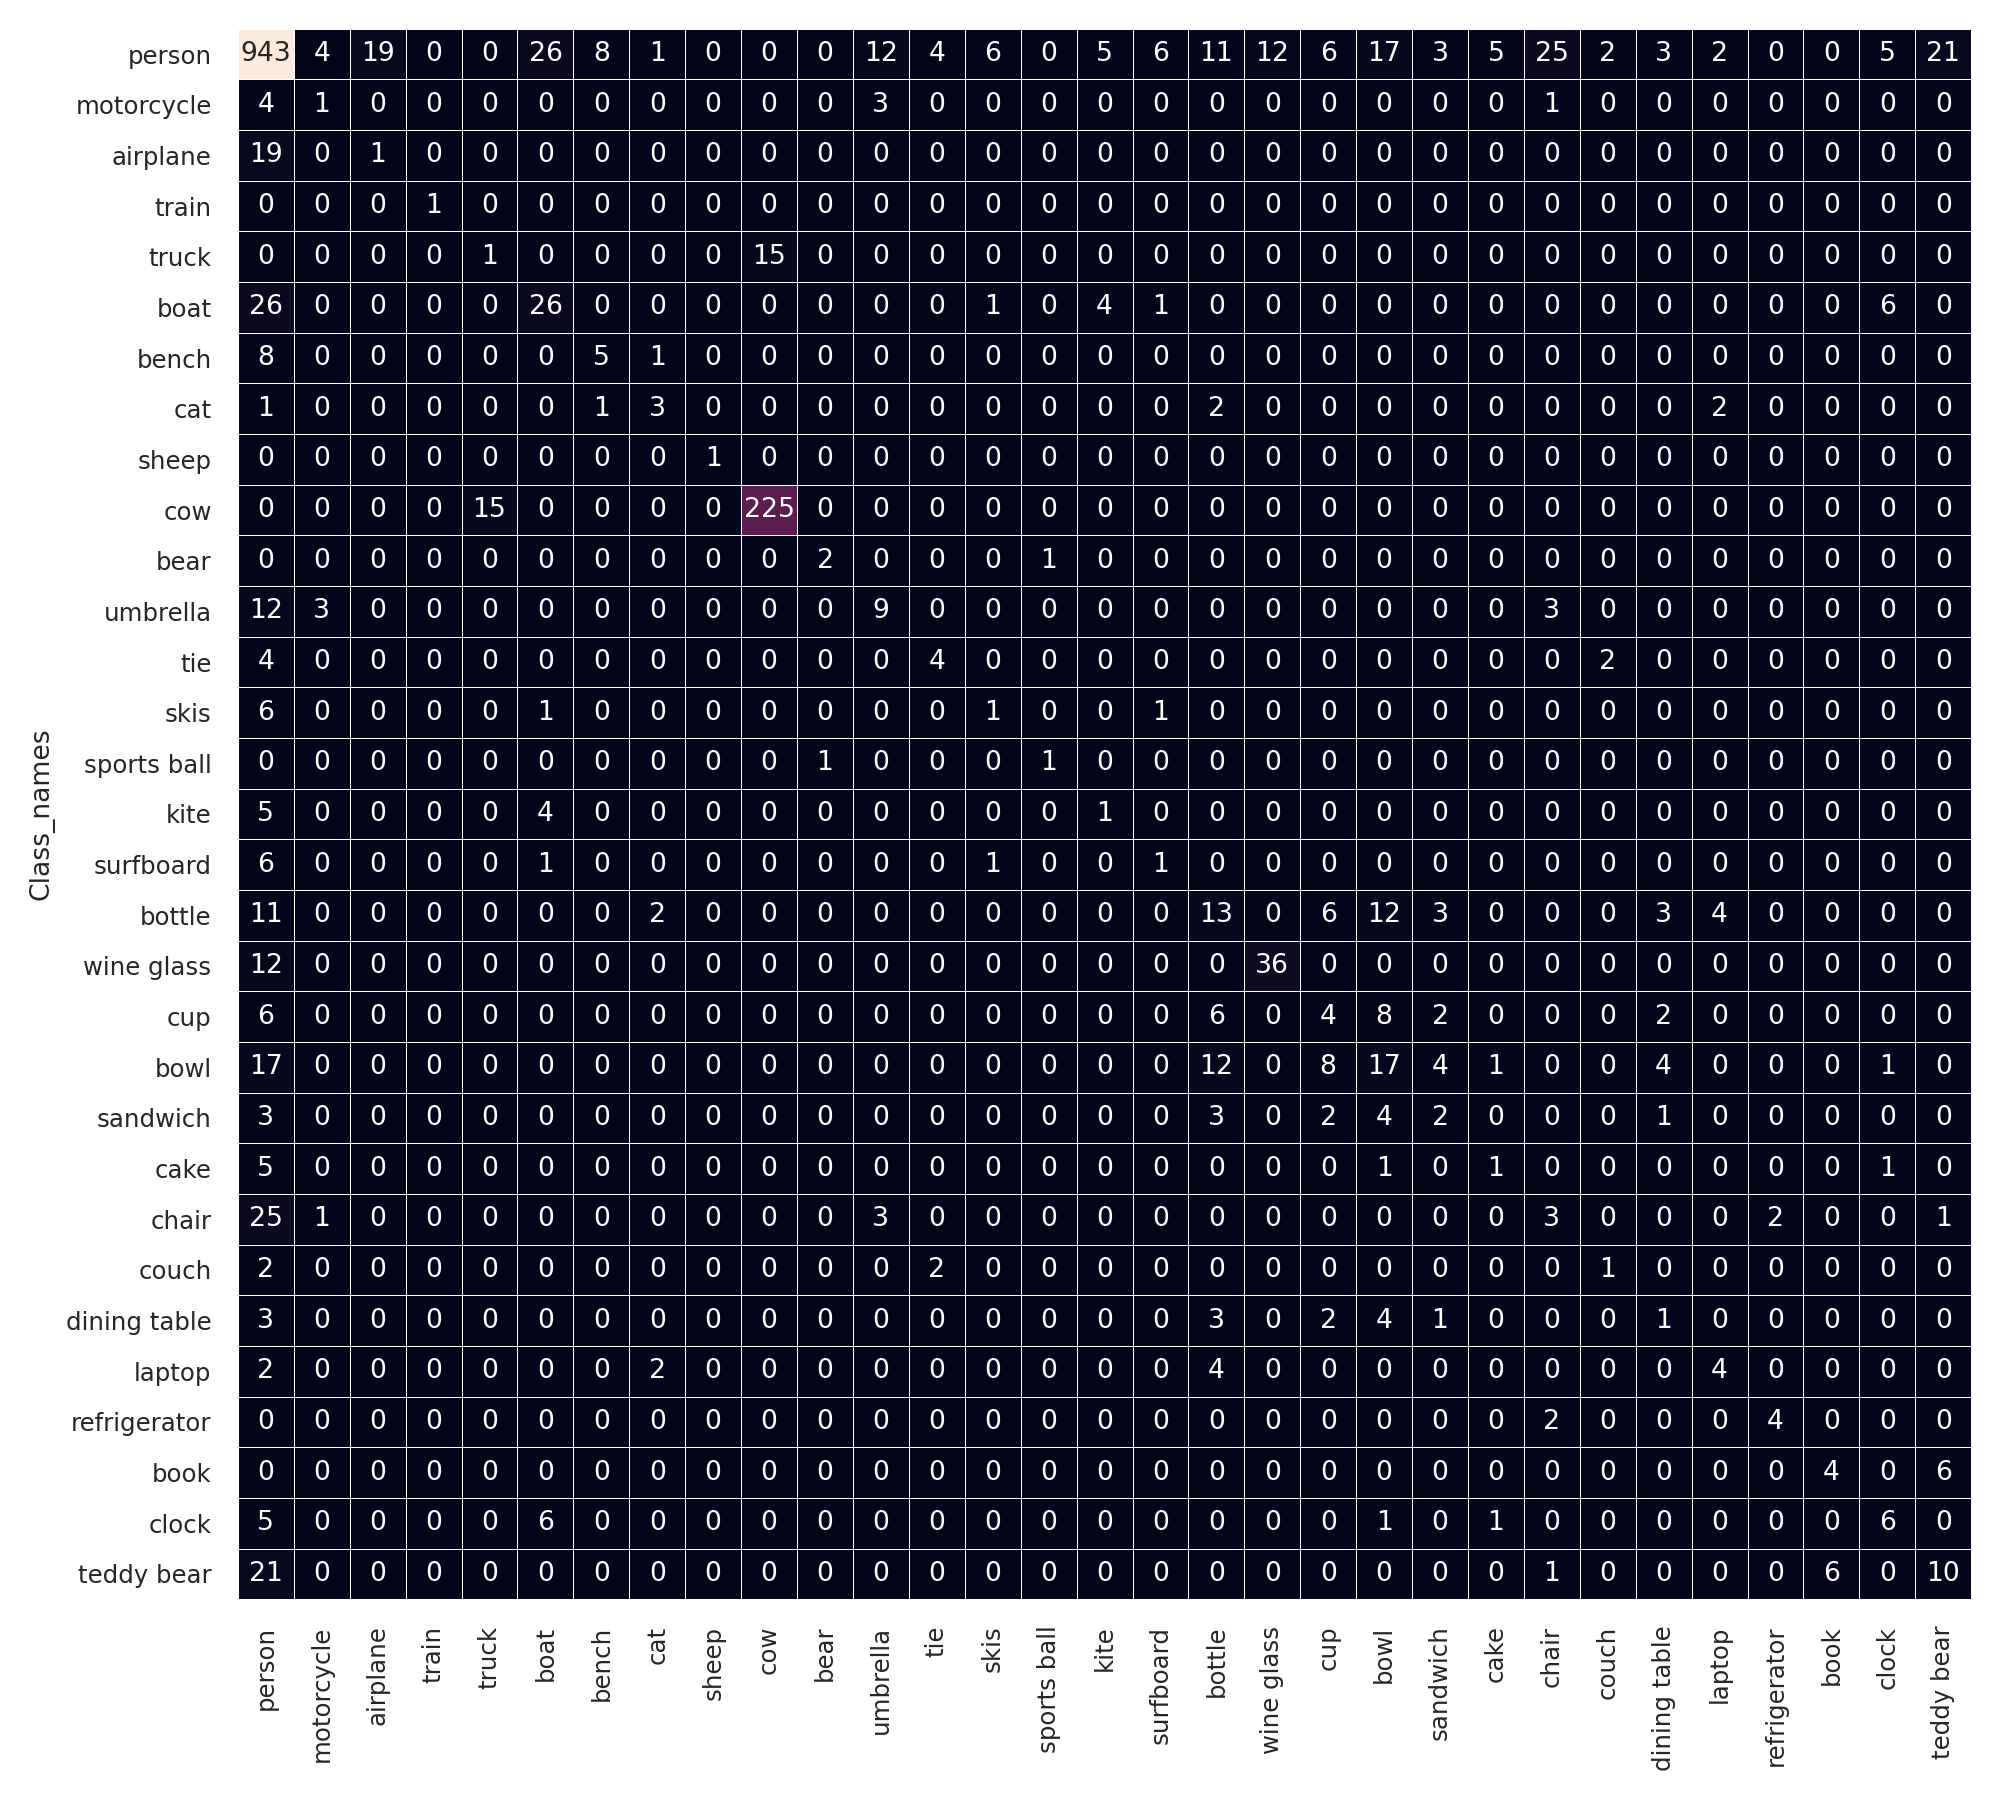
\includegraphics[width=\textwidth,height=\textheight,keepaspectratio]{Resources/Images/task_a_cooc.png}
    \caption{Task A: Co-occurrence matrix.}
    \label{fig:task_a_cooc}
\end{figure}


\begin{figure}[hbt]
    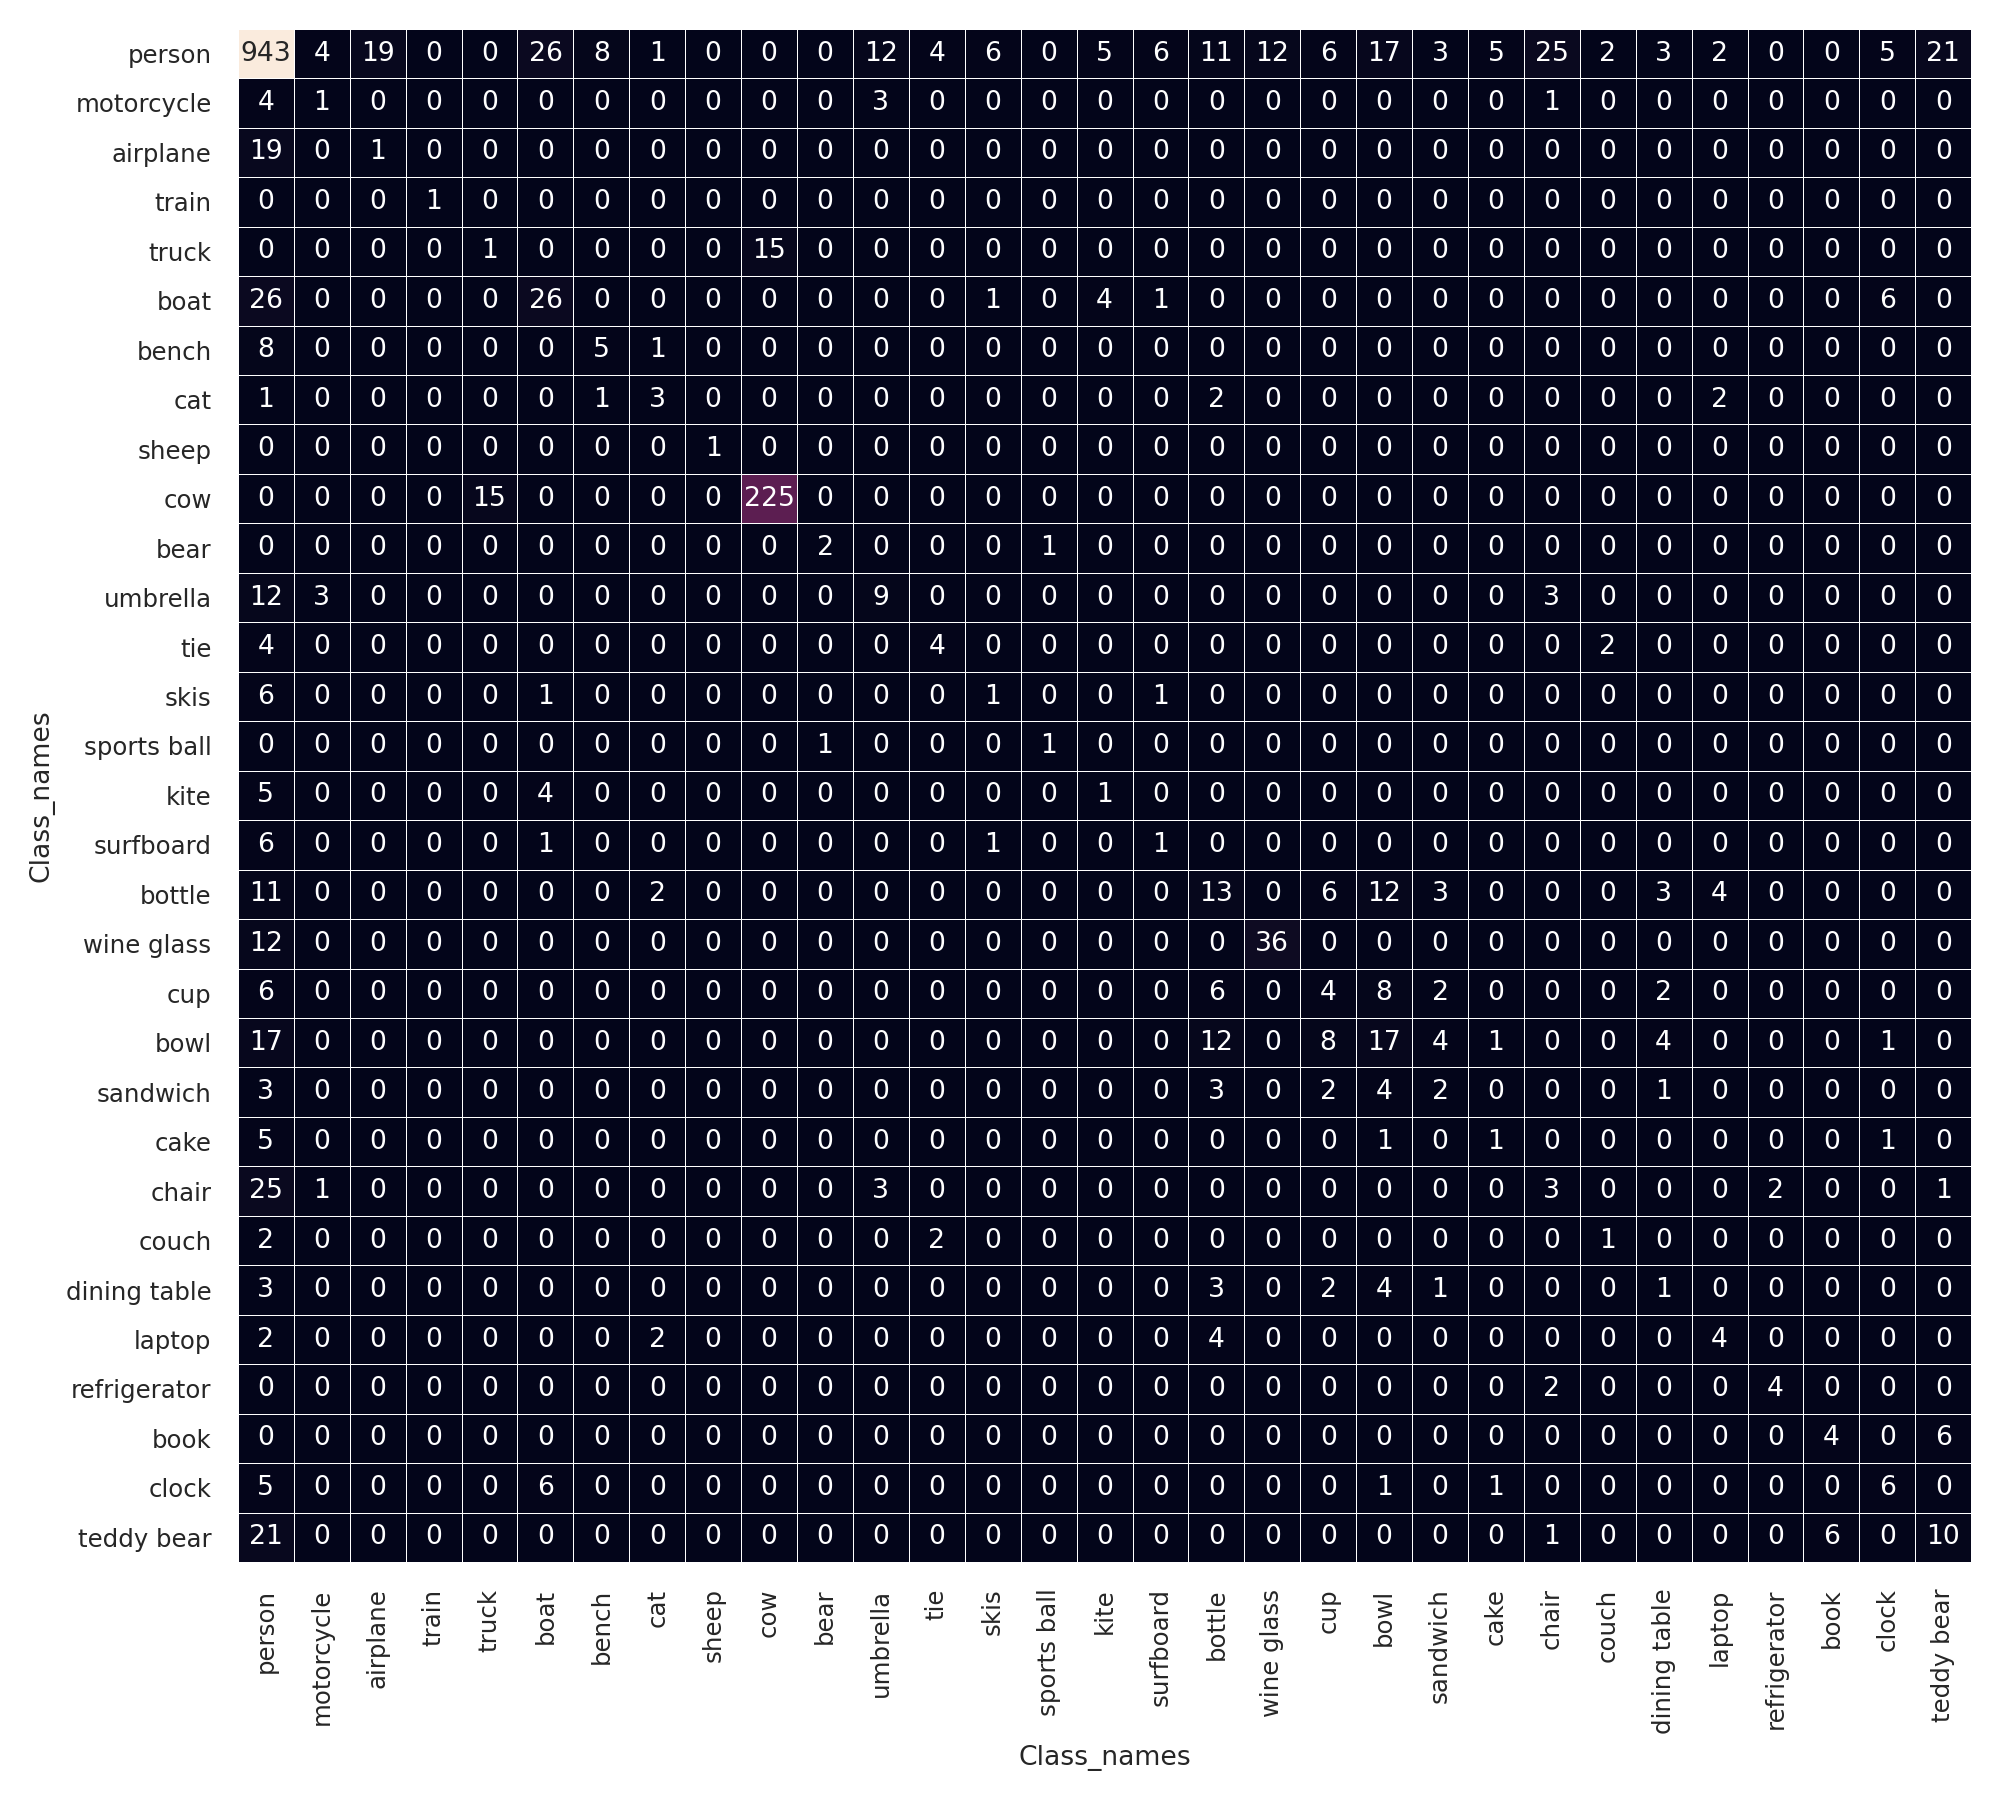
\includegraphics[width=\textwidth,height=\textheight,keepaspectratio]{Resources/Images/task_b_cooc.png}
    \caption{Task B Co-occurrence matrix.}
    \label{fig:task_b_cooc}
\end{figure}

\begin{figure}[hbt]
    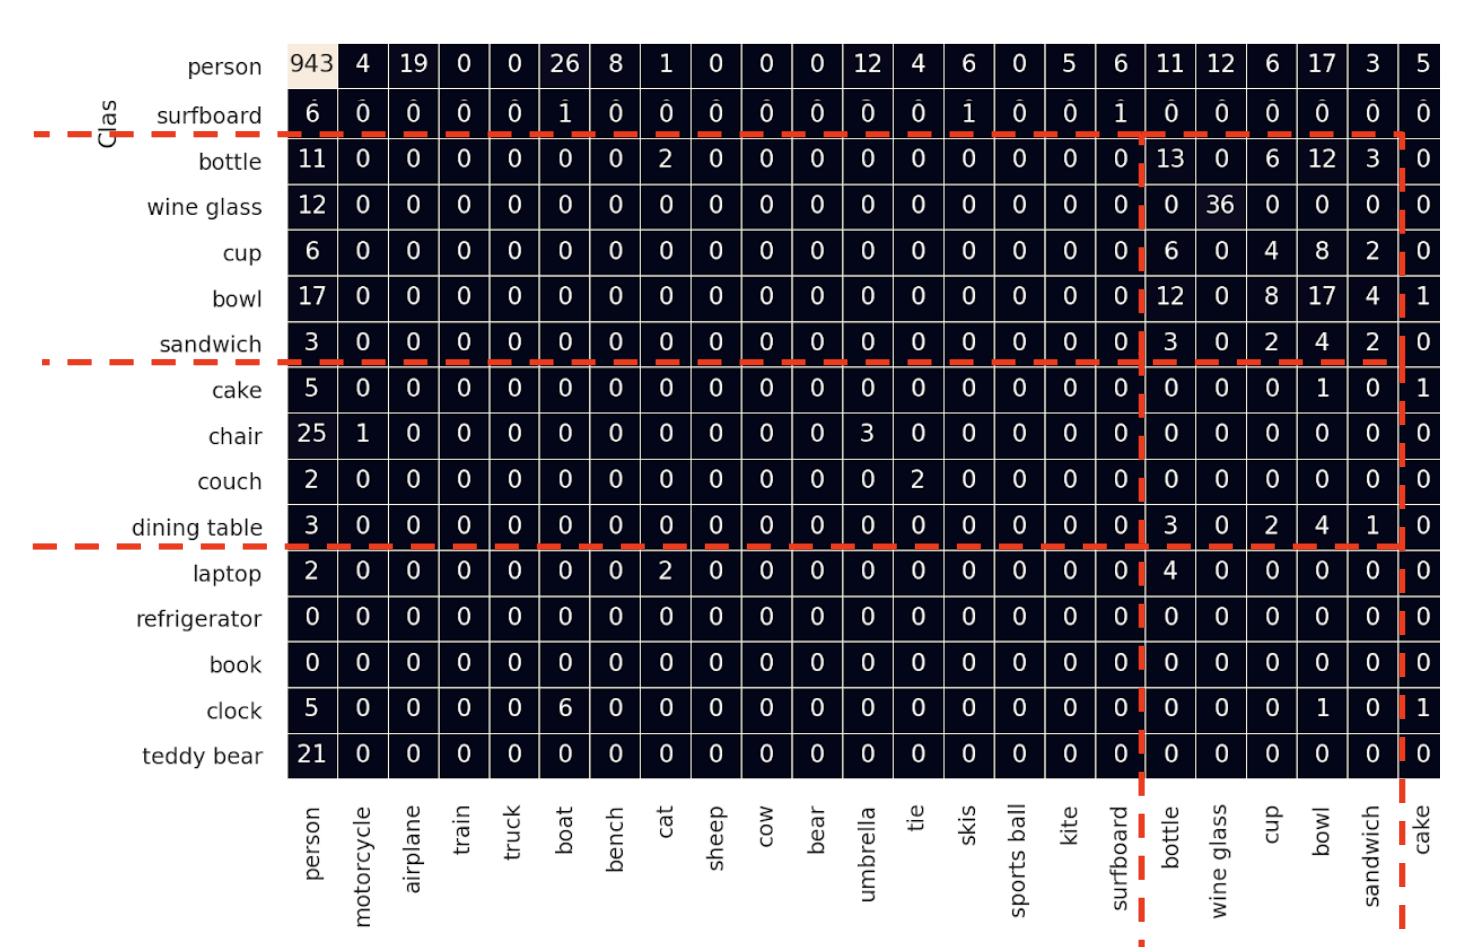
\includegraphics[width=\textwidth,height=\textheight,keepaspectratio]{Resources/Images/task_b_interesting.png}
    \caption{Task B: Interesting co-occurrences.}
    \label{fig:task_b_interesting}
\end{figure}

\begin{figure}[hbt]
    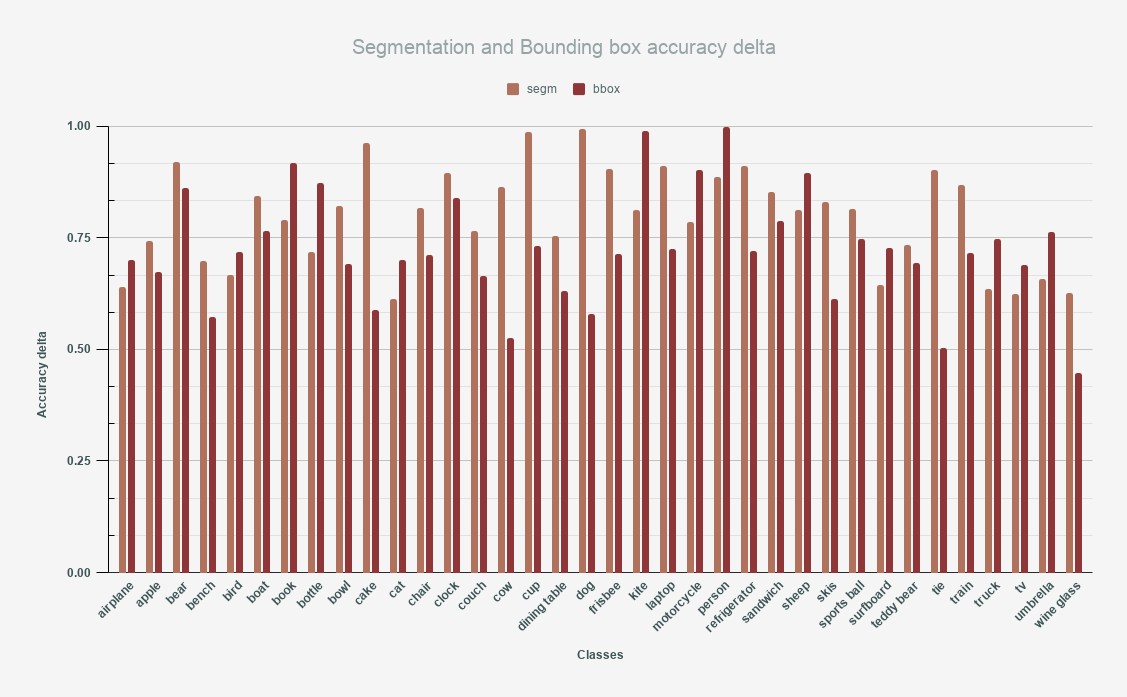
\includegraphics[width=\textwidth,height=\textheight,keepaspectratio]{Resources/Images/task_b_deltas.png}
    \caption{Task B: Accuracy delta.}
    \label{fig:task_b_deltas}
\end{figure}


\begin{figure}[hbt]
    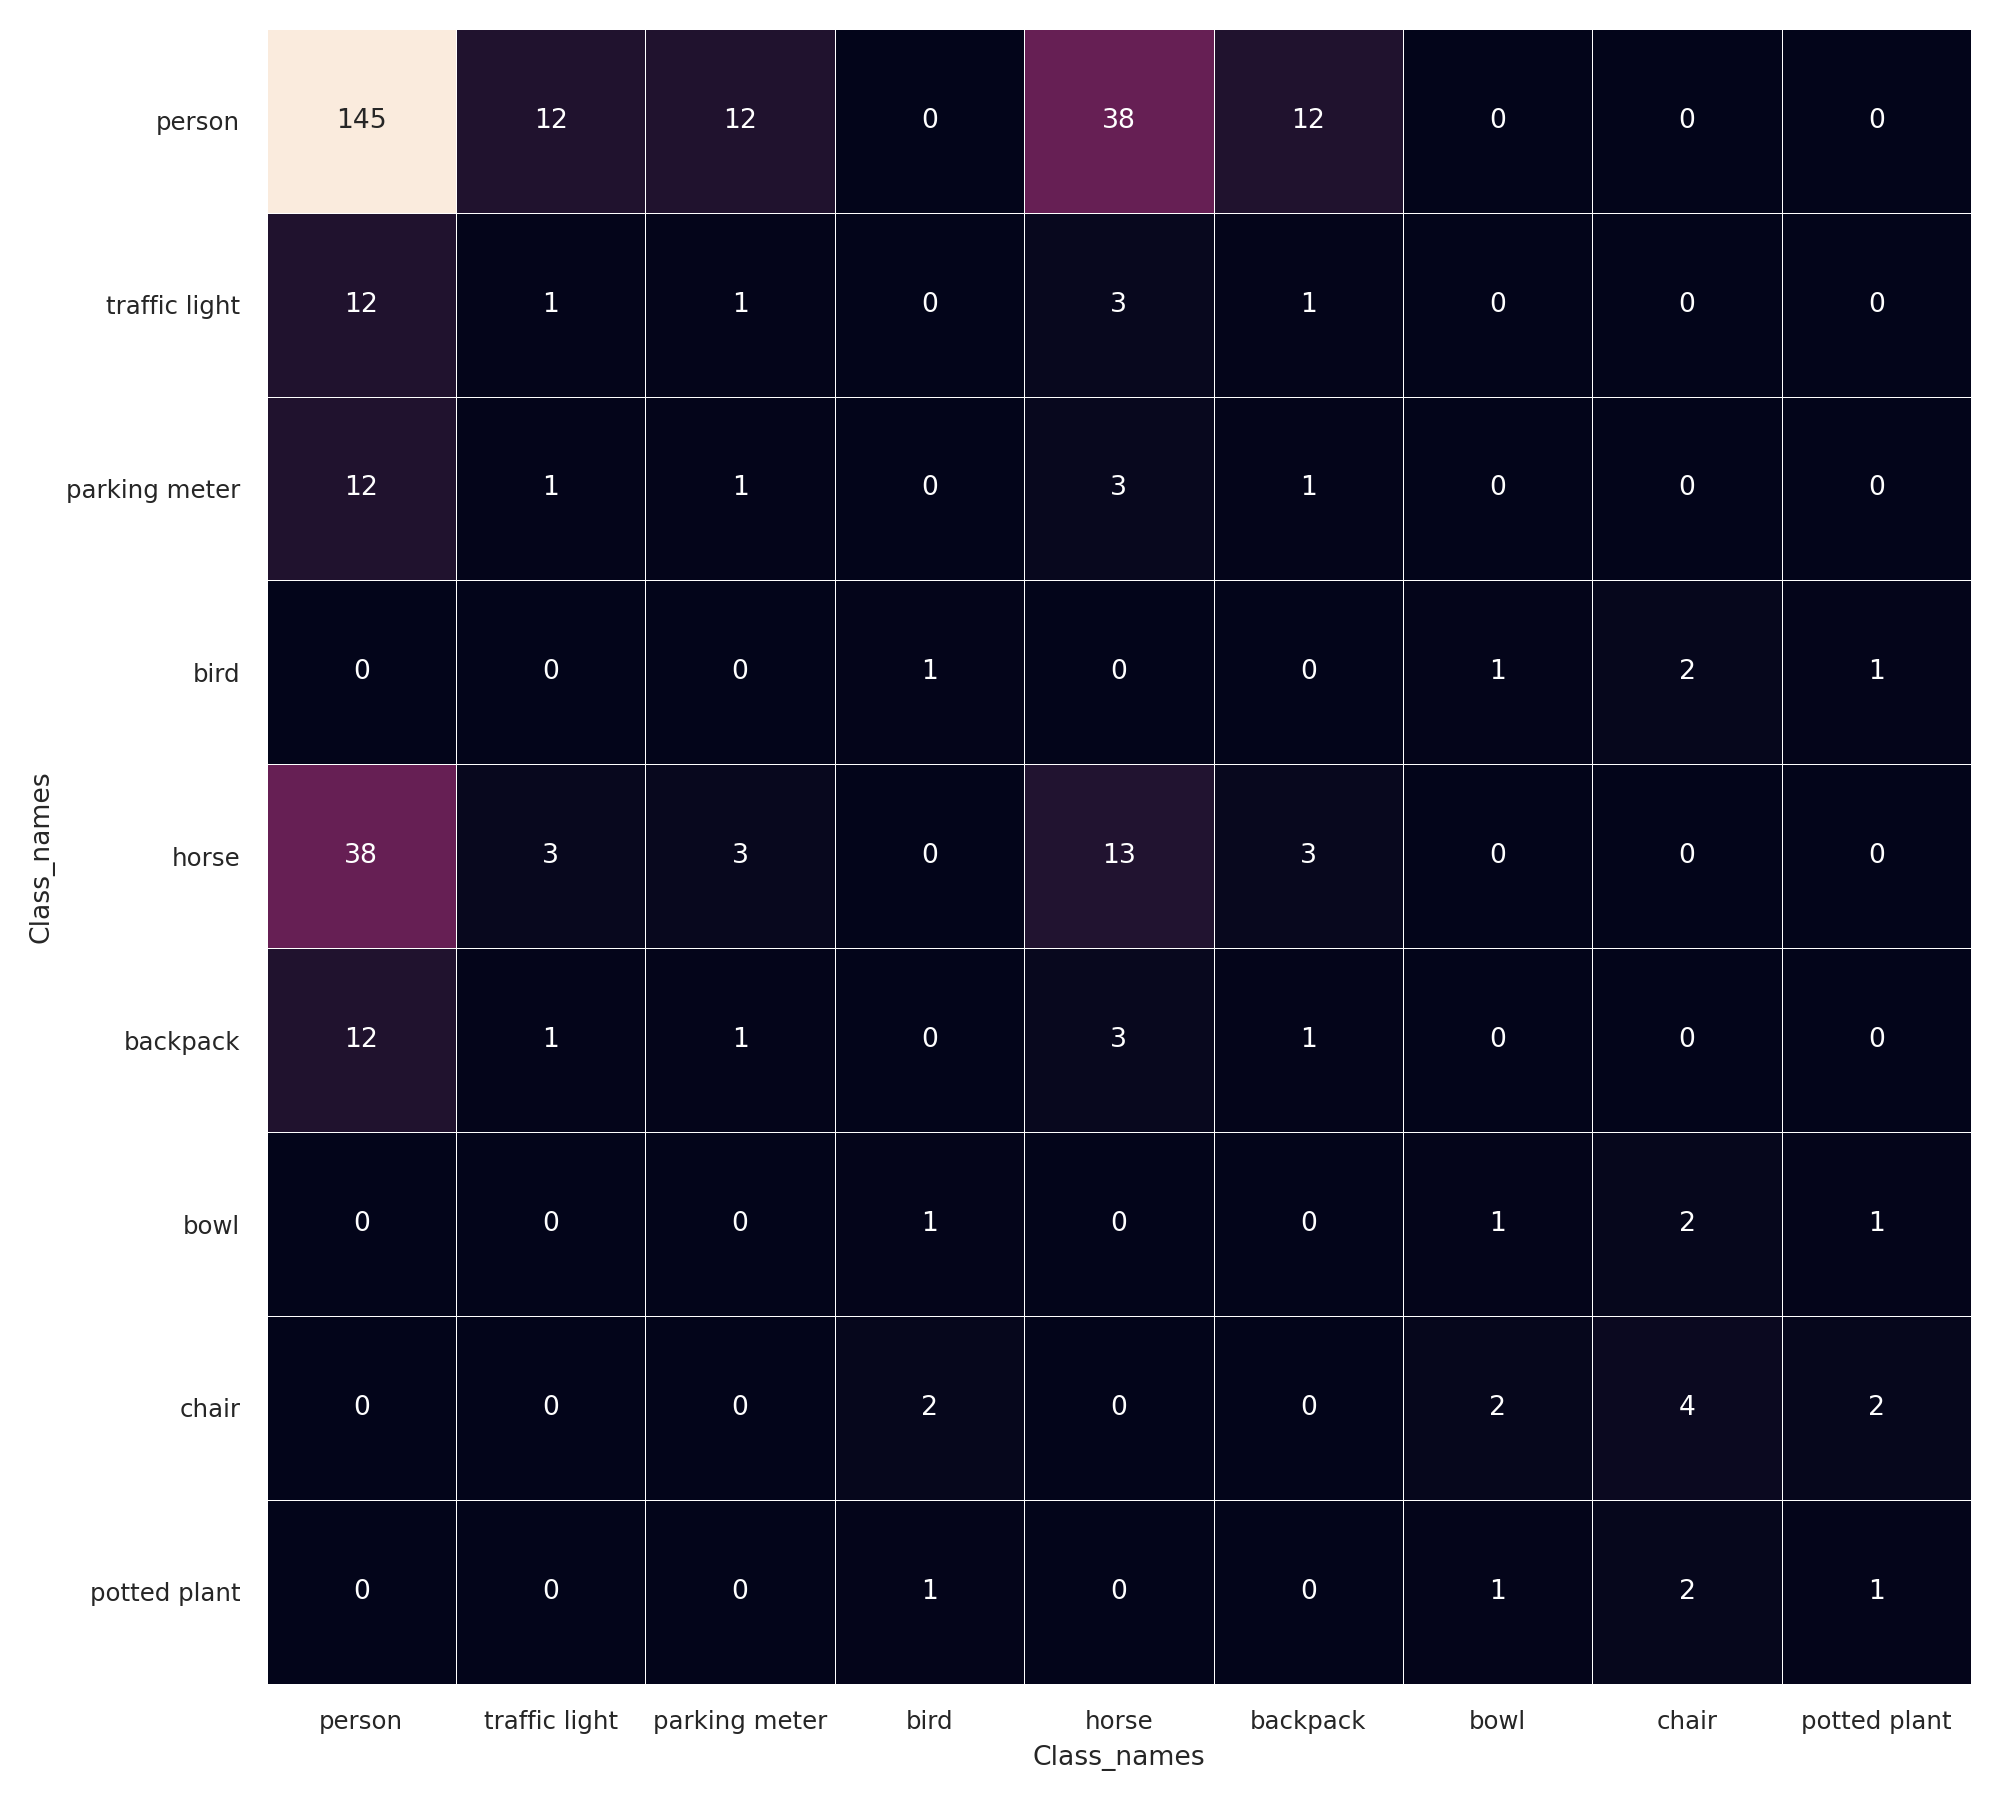
\includegraphics[width=\textwidth,height=\textheight,keepaspectratio]{Resources/Images/task_c_orig_.png}
    \caption{Task C: Original images co-occurrence matrix.}
    \label{fig:task_c_orig}
\end{figure}


\begin{figure}[hbt]
    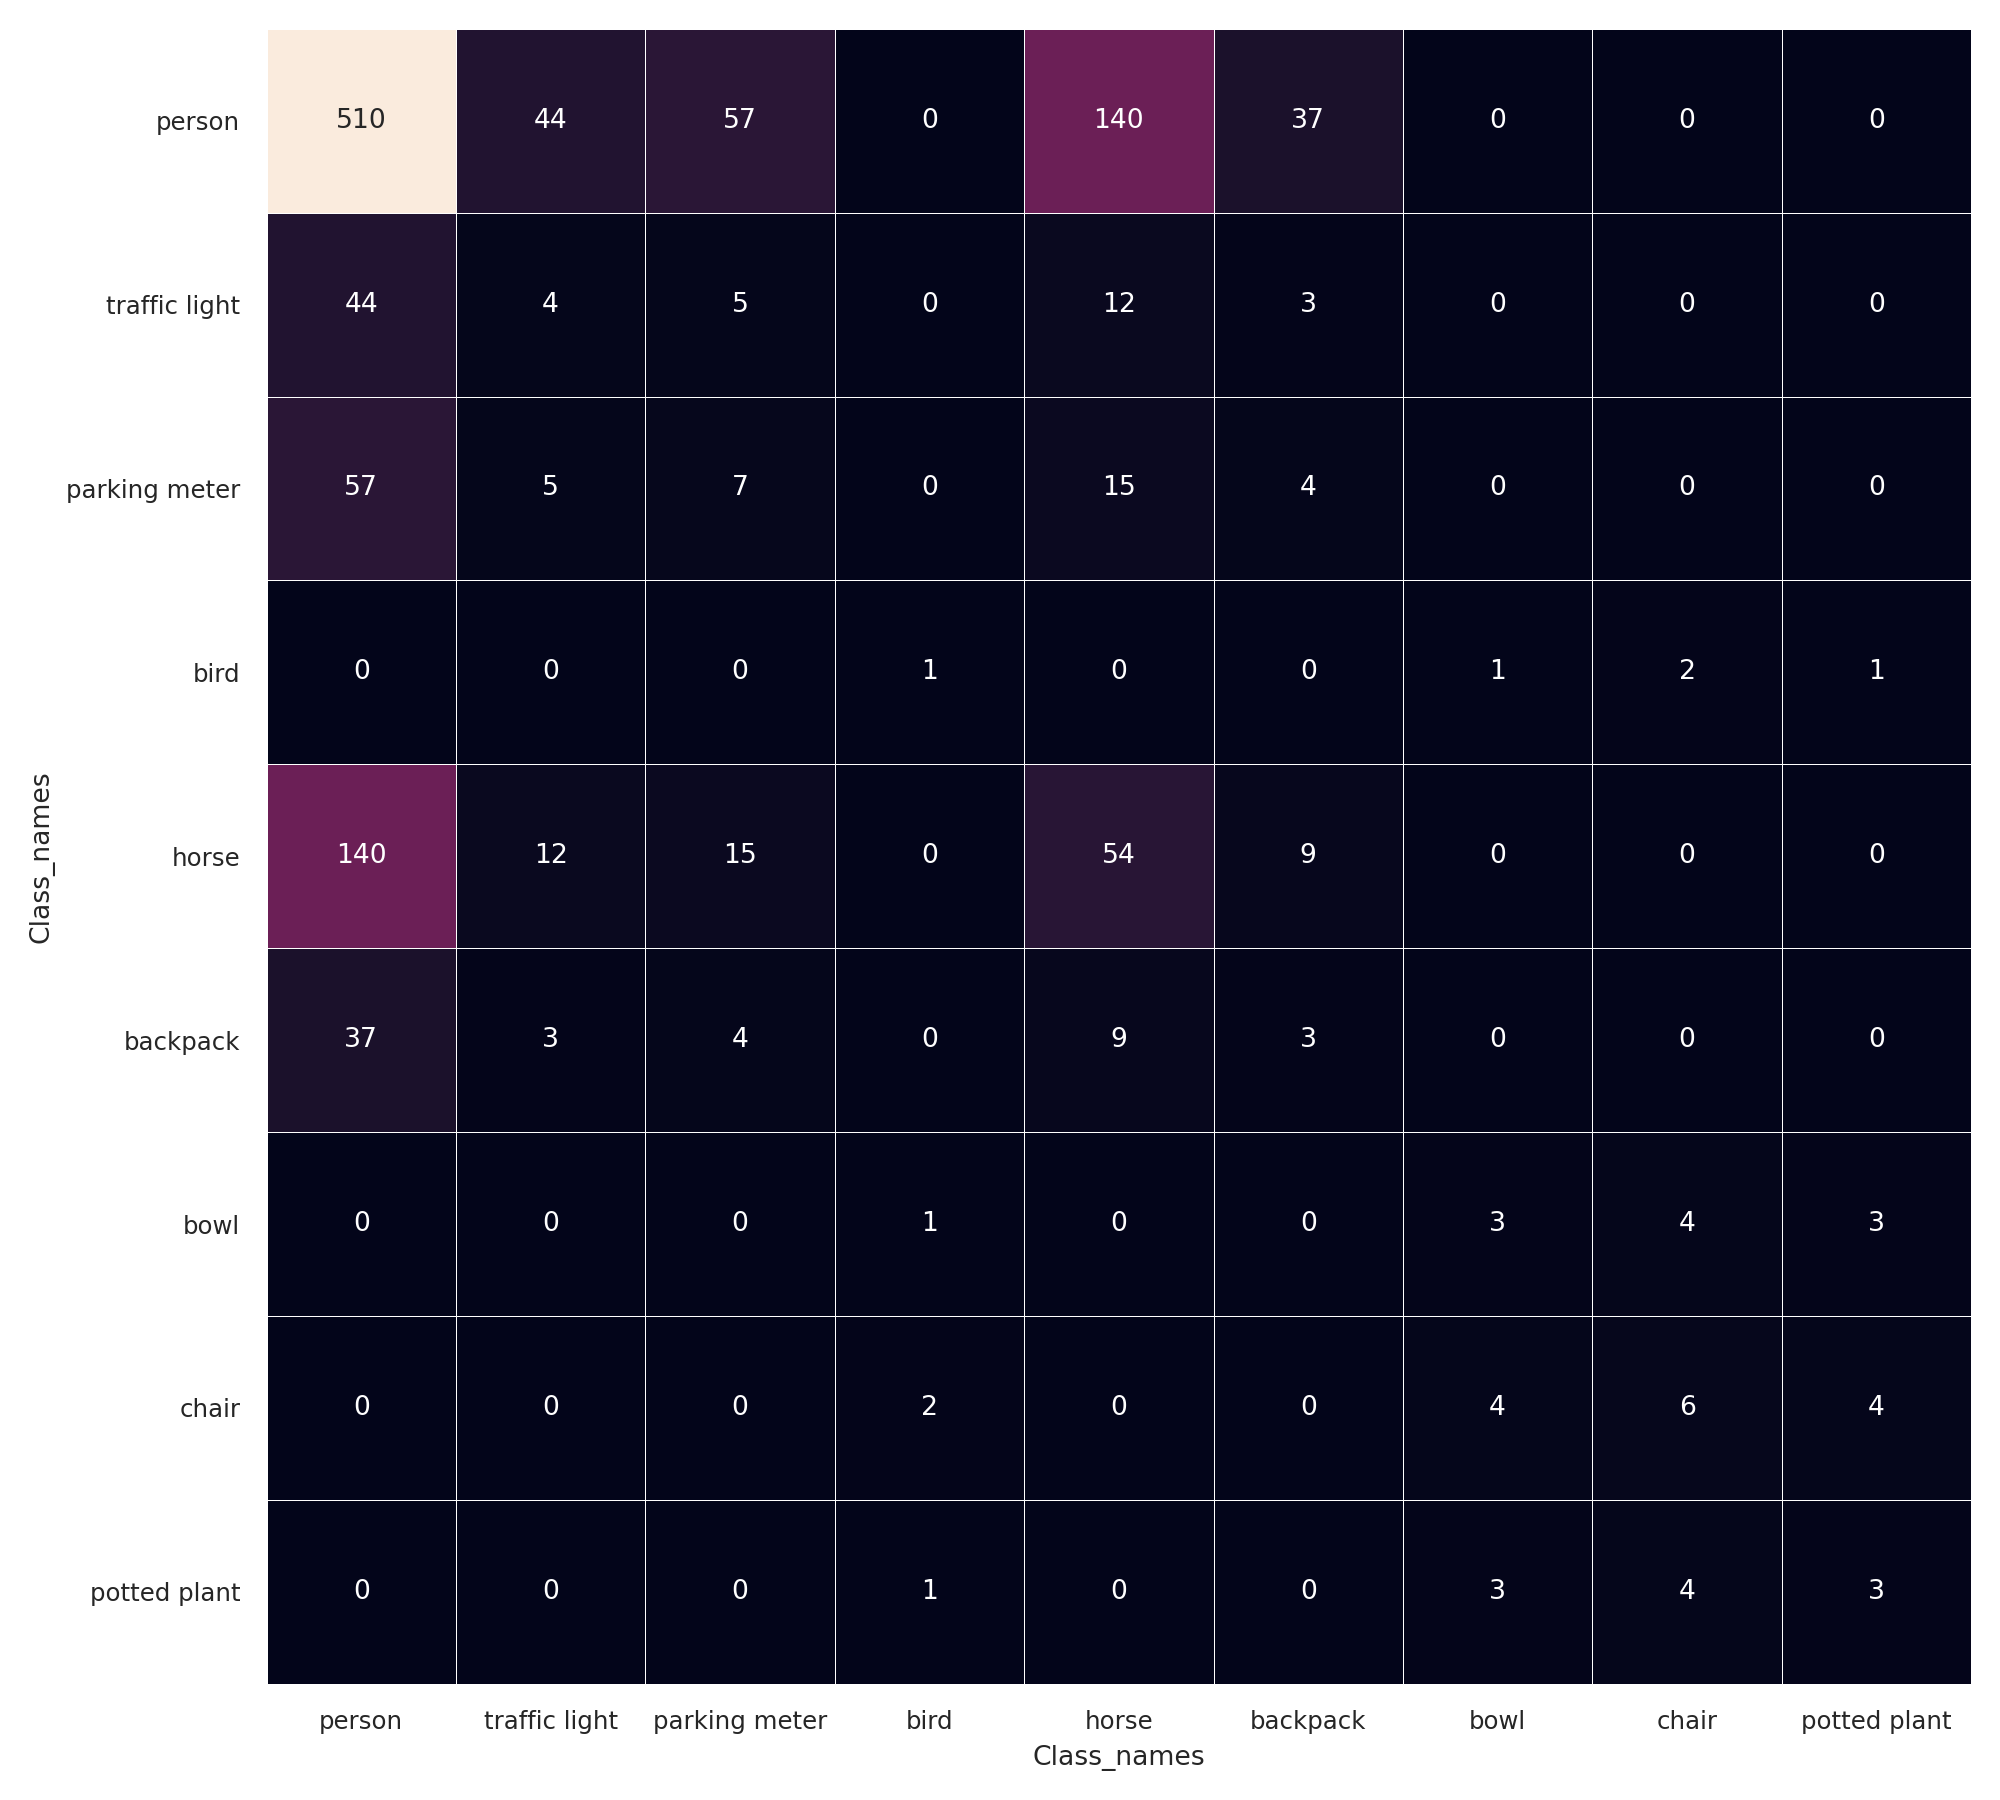
\includegraphics[width=\textwidth,height=\textheight,keepaspectratio]{Resources/Images/task_c_mods_.png}
    \caption{Task C: Modified images co-occurrence matrix.}
    \label{fig:task_c_mod}
\end{figure}

\begin{figure}[hbt]
    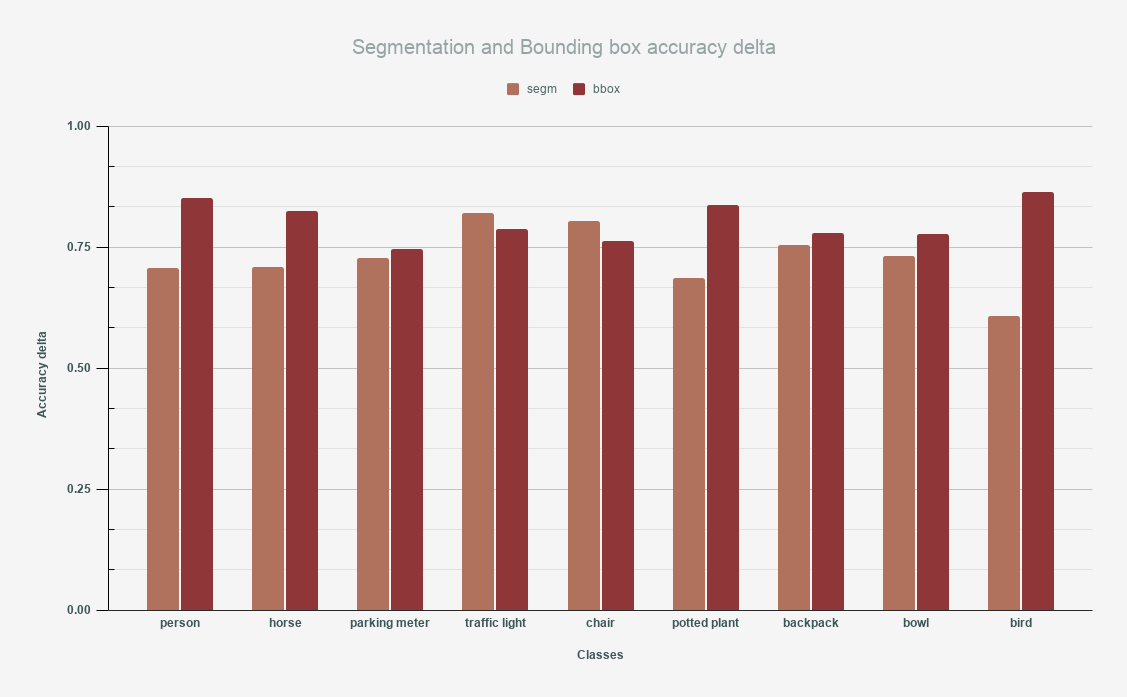
\includegraphics[width=\textwidth,height=\textheight,keepaspectratio]{Resources/Images/task_c_deltas.png}
    \caption{Task C: Accuracy deltas.}
    \label{fig:task_c_deltas}
\end{figure}

\begin{figure}[hbt]
    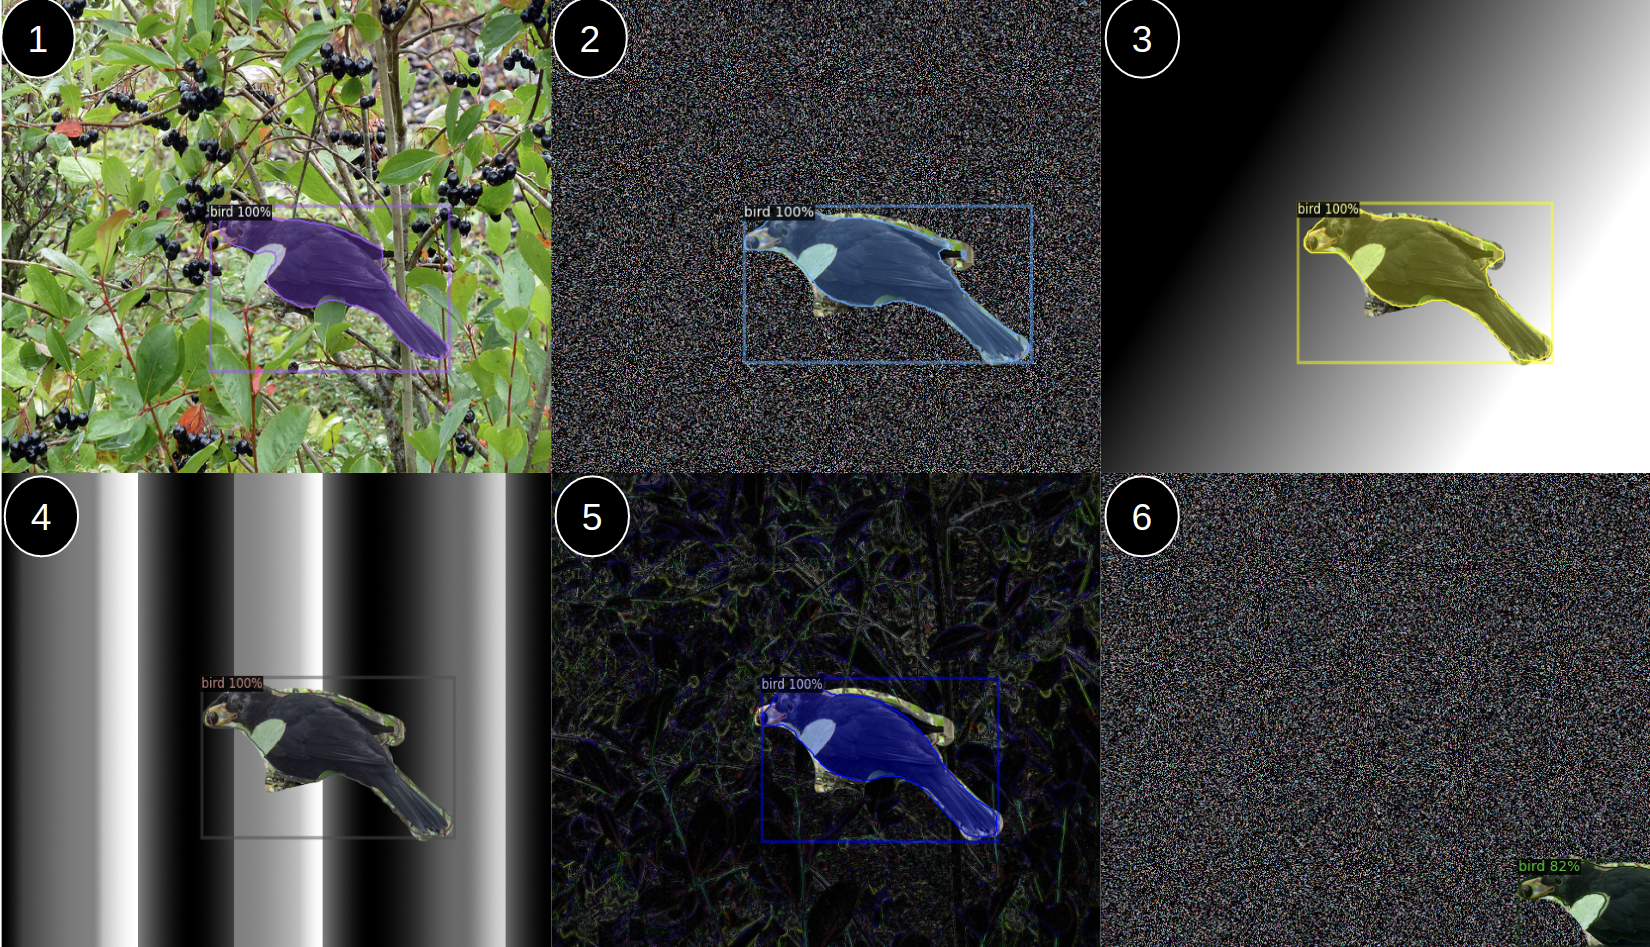
\includegraphics[width=\textwidth,height=\textheight,keepaspectratio]{Resources/Images/task_c_bird.png}
    \caption{Task D: A Bird.}
    \label{fig:task_d_bird}
\end{figure}

\begin{figure}[hbt]
    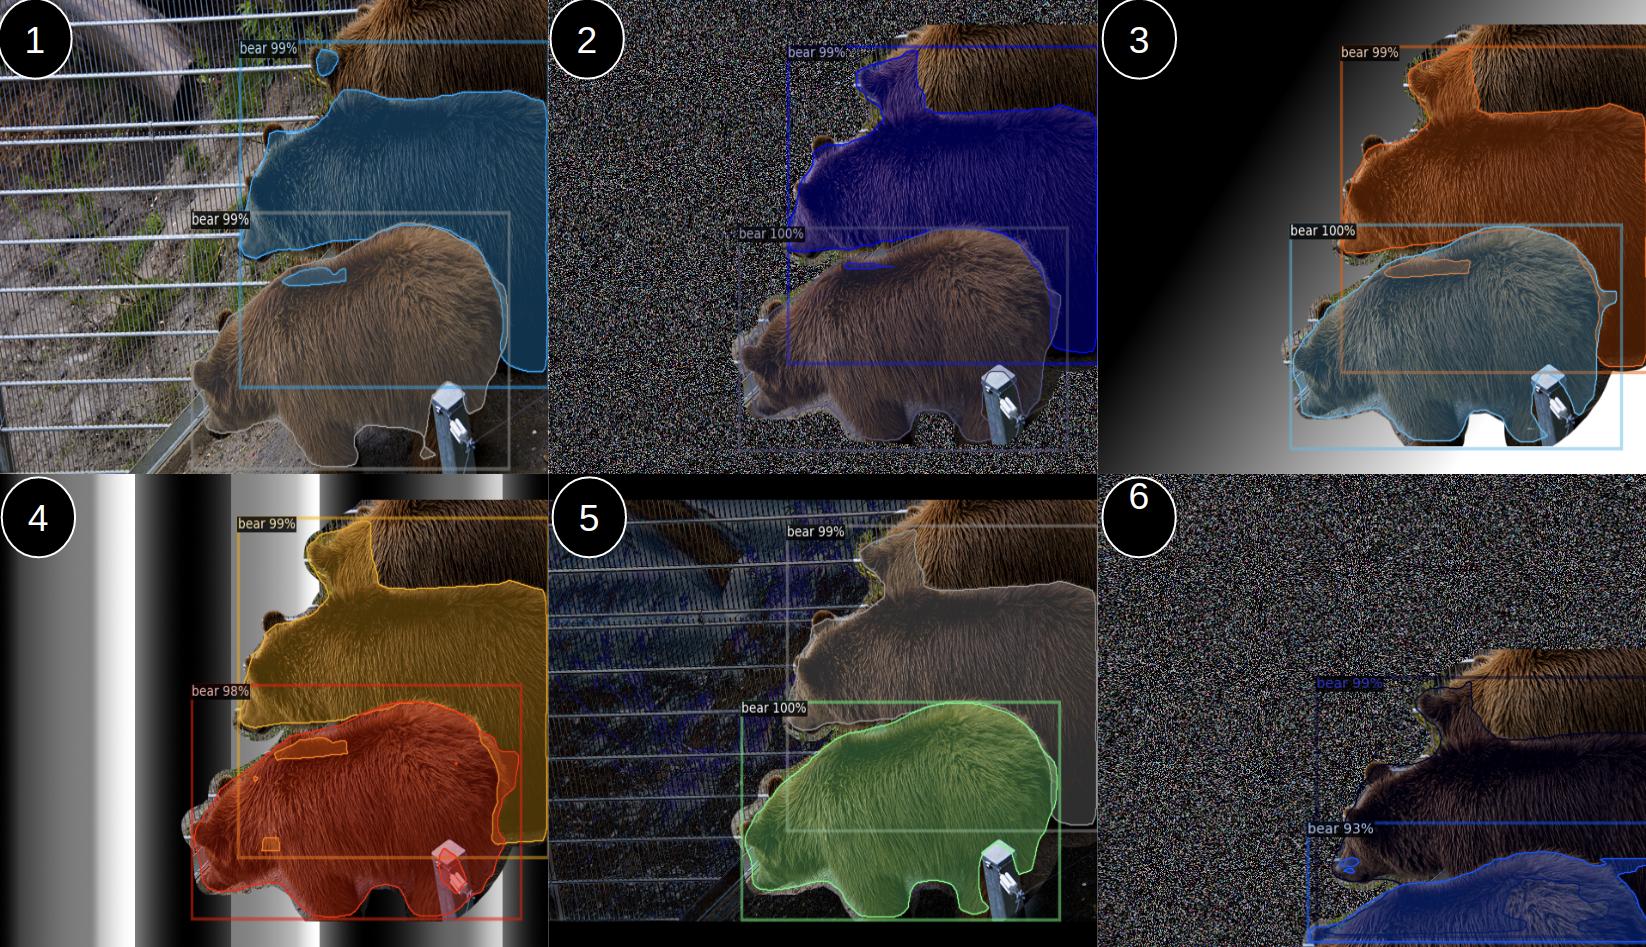
\includegraphics[width=\textwidth,height=\textheight,keepaspectratio]{Resources/Images/task_c_bear.png}
    \caption{Task D: A Bear.}
    \label{fig:task_d_bear}
\end{figure}

\begin{figure}[hbt]
    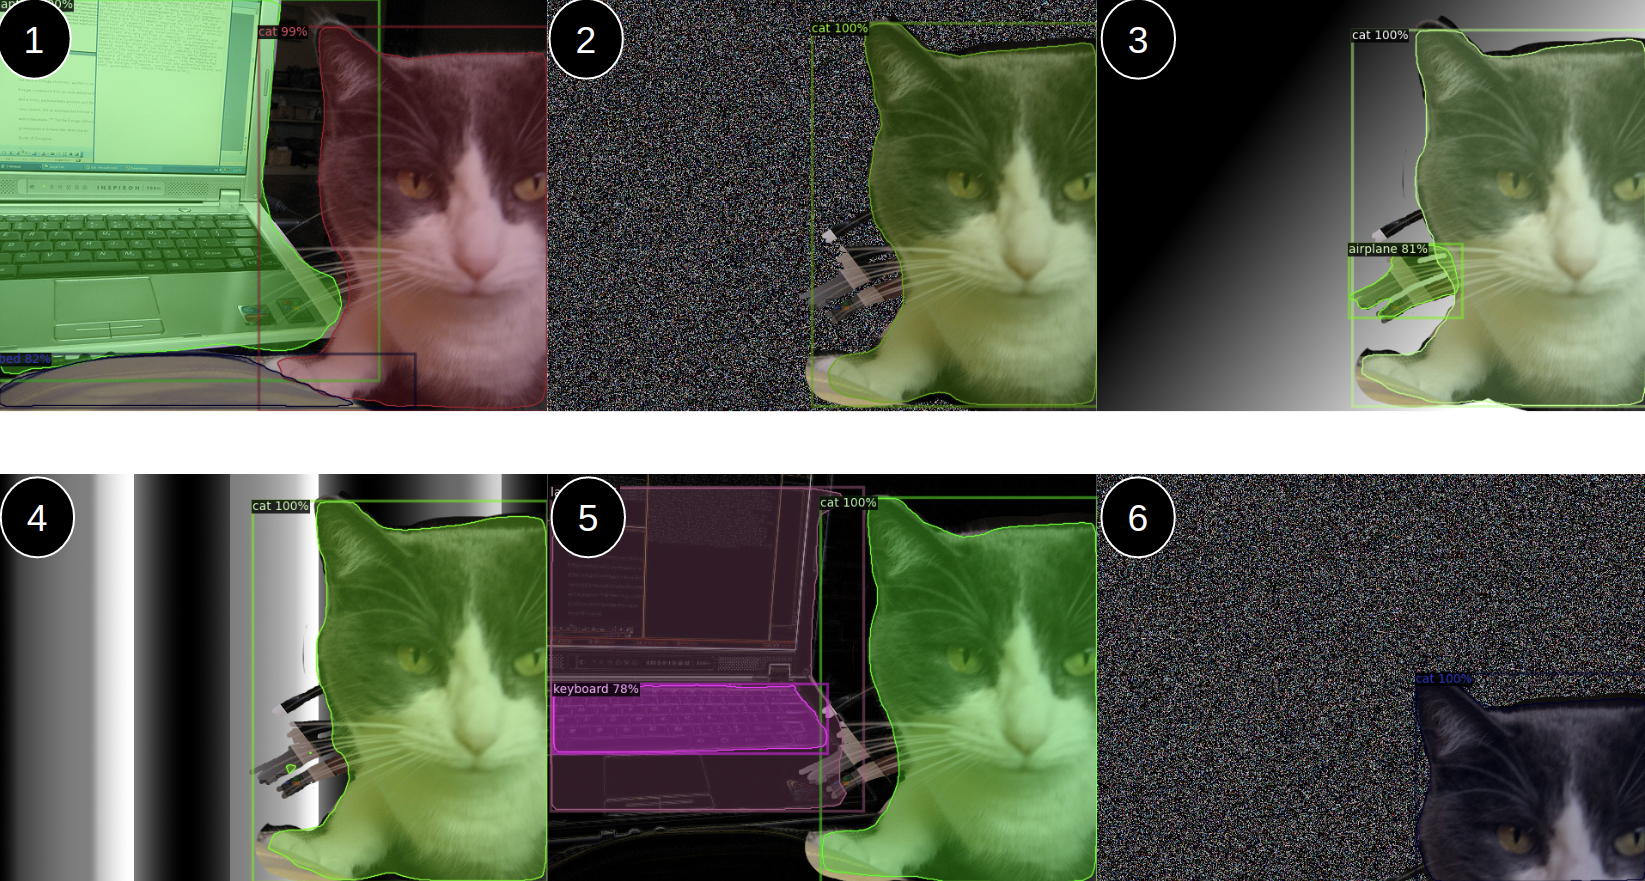
\includegraphics[width=\textwidth,height=\textheight,keepaspectratio]{Resources/Images/task_c_cat.png}
    \caption{Task D: A Cat.}
    \label{fig:task_d_cat}
\end{figure}


\end{document}
